% Template for PLoS
% Version 3.5 March 2018
%
% % % % % % % % % % % % % % % % % % % % % %
%
% -- IMPORTANT NOTE
%
% This template contains comments intended
% to minimize problems and delays during our production
% process. Please follow the template instructions
% whenever possible.
%
% % % % % % % % % % % % % % % % % % % % % % %
%
% Once your paper is accepted for publication,
% PLEASE REMOVE ALL TRACKED CHANGES in this file
% and leave only the final text of your manuscript.
% PLOS recommends the use of latexdiff to track changes during review, as this will help to maintain a clean tex file.
% Visit https://www.ctan.org/pkg/latexdiff?lang=en for info or contact us at latex@plos.org.
%
%
% There are no restrictions on package use within the LaTeX files except that
% no packages listed in the template may be deleted.
%
% Please do not include colors or graphics in the text.
%
% The manuscript LaTeX source should be contained within a single file (do not use \input, \externaldocument, or similar commands).
%
% % % % % % % % % % % % % % % % % % % % % % %
%
% -- FIGURES AND TABLES
%
% Please include tables/figure captions directly after the paragraph where they are first cited in the text.
%
% DO NOT INCLUDE GRAPHICS IN YOUR MANUSCRIPT
% - Figures should be uploaded separately from your manuscript file.
% - Figures generated using LaTeX should be extracted and removed from the PDF before submission.
% - Figures containing multiple panels/subfigures must be combined into one image file before submission.
% For figure citations, please use "Fig" instead of "Figure".
% See http://journals.plos.org/plosone/s/figures for PLOS figure guidelines.
%
% Tables should be cell-based and may not contain:
% - spacing/line breaks within cells to alter layout or alignment
% - do not nest tabular environments (no tabular environments within tabular environments)
% - no graphics or colored text (cell background color/shading OK)
% See http://journals.plos.org/plosone/s/tables for table guidelines.
%
% For tables that exceed the width of the text column, use the adjustwidth environment as illustrated in the example table in text below.
%
% % % % % % % % % % % % % % % % % % % % % % % %
%
% -- EQUATIONS, MATH SYMBOLS, SUBSCRIPTS, AND SUPERSCRIPTS
%
% IMPORTANT
% Below are a few tips to help format your equations and other special characters according to our specifications. For more tips to help reduce the possibility of formatting errors during conversion, please see our LaTeX guidelines at http://journals.plos.org/plosone/s/latex
%
% For inline equations, please be sure to include all portions of an equation in the math environment.  For example, x$^2$ is incorrect; this should be formatted as $x^2$ (or $\mathrm{x}^2$ if the romanized font is desired).
%
% Do not include text that is not math in the math environment. For example, CO2 should be written as CO\textsubscript{2} instead of CO$_2$.
%
% Please add line breaks to long display equations when possible in order to fit size of the column.
%
% For inline equations, please do not include punctuation (commas, etc) within the math environment unless this is part of the equation.
%
% When adding superscript or subscripts outside of brackets/braces, please group using {}.  For example, change "[U(D,E,\gamma)]^2" to "{[U(D,E,\gamma)]}^2".
%
% Do not use \cal for caligraphic font.  Instead, use \mathcal{}
%
% % % % % % % % % % % % % % % % % % % % % % % %
%
% Please contact latex@plos.org with any questions.
%
% % % % % % % % % % % % % % % % % % % % % % % %

\documentclass[10pt,letterpaper]{article}
\usepackage[top=0.85in,left=2.75in,footskip=0.75in]{geometry}

% amsmath and amssymb packages, useful for mathematical formulas and symbols
\usepackage{amsmath,amssymb}

% Use adjustwidth environment to exceed column width (see example table in text)
\usepackage{changepage}

% Use Unicode characters when possible
\usepackage[utf8x]{inputenc}

% textcomp package and marvosym package for additional characters
\usepackage{textcomp,marvosym}

% cite package, to clean up citations in the main text. Do not remove.
\usepackage{cite}

% Use nameref to cite supporting information files (see Supporting Information section for more info)
\usepackage{nameref,hyperref}
\usepackage[capitalize]{cleveref}
\crefformat{equation}{Eq~(#2#1#3)}
\crefrangeformat{equation}{Eqs~(#3#1#4) to~(#5#2#6)}
\crefmultiformat{equation}{Eqs~(#2#1#3)}%
{ and~(#2#1#3)}{, (#2#1#3)}{ and~(#2#1#3)}
\crefformat{figure}{Fig~#2#1#3}
\crefrangeformat{figure}{Figs~#3#1#4 to~#5#2#6}
\crefmultiformat{figure}{Figs~#2#1#3}%
{ and~#2#1#3}{, #2#1#3}{ and~#2#1#3}

\usepackage[inline]{enumitem}
\usepackage[per-mode=symbol,group-separator={,},group-minimum-digits=4]{siunitx}
\usepackage{listings}
\usepackage{todonotes}
\usepackage{subcaption}
\usepackage{url}

\lstset{basicstyle=\ttfamily}

% color can be used to apply background shading to table cells only
\usepackage{xcolor}

\usepackage[commentmarkup=footnote]{changes}

% line numbers
\usepackage[right]{lineno}

% ligatures disabled
\usepackage{microtype}
\DisableLigatures[f]{encoding = *, family = * }

% array package and thick rules for tables
\usepackage{array}

\usepackage{physics}  % for \norm
\usepackage{graphicx}
\graphicspath{ {../paper_figures} }

% create "+" rule type for thick vertical lines
\newcolumntype{+}{!{\vrule width 2pt}}

% create \thickcline for thick horizontal lines of variable length
\newlength\savedwidth
\newcommand\thickcline[1]{%
  \noalign{\global\savedwidth\arrayrulewidth\global\arrayrulewidth 2pt}%
  \cline{#1}%
  \noalign{\vskip\arrayrulewidth}%
  \noalign{\global\arrayrulewidth\savedwidth}%
}

% \thickhline command for thick horizontal lines that span the table
\newcommand\thickhline{\noalign{\global\savedwidth\arrayrulewidth\global\arrayrulewidth 2pt}%
\hline
\noalign{\global\arrayrulewidth\savedwidth}}

% Remove comment for double spacing
%\usepackage{setspace}
%\doublespacing

% Text layout
\raggedright
\setlength{\parindent}{0.5cm}
\textwidth 5.25in
\textheight 8.75in

% Bold the 'Figure #' in the caption and separate it from the title/caption with a period
% Captions will be left justified
\usepackage[aboveskip=1pt,labelfont=bf,labelsep=period,justification=raggedright,singlelinecheck=off]{caption}
\renewcommand{\figurename}{Fig}

% Use the PLoS provided BiBTeX style
\bibliographystyle{plos2015}

% Remove brackets from numbering in List of References
\makeatletter
\renewcommand{\@biblabel}[1]{\quad#1.}
\makeatother


% Header and Footer with logo
\usepackage{lastpage,fancyhdr,graphicx}
\usepackage{epstopdf}
%\pagestyle{myheadings}
\pagestyle{fancy}
\fancyhf{}
%\setlength{\headheight}{27.023pt}
%\lhead{\includegraphics[width=2.0in]{PLOS-submission.eps}}
\rfoot{\thepage/\pageref{LastPage}}
\renewcommand{\headrulewidth}{0pt}
\renewcommand{\footrule}{\hrule height 2pt \vspace{2mm}}
\fancyheadoffset[L]{2.25in}
\fancyfootoffset[L]{2.25in}
\lfoot{\today}

%% Include all macros below

\newcommand{\lorem}{{\bf LOREM}}
\newcommand{\ipsum}{{\bf IPSUM}}

%% END MACROS SECTION

\begin{document}
\vspace*{0.2in}

% Title must be 250 characters or less.
\begin{flushleft}
{\Large
\textbf\newline{Multidimensional analysis and detection of informative features in human brain white matter} % Please use "sentence case" for title and headings (capitalize only the first word in a title (or heading), the first word in a subtitle (or subheading), and any proper nouns).
}
\newline
% Insert author names, affiliations and corresponding author email (do not include titles, positions, or degrees).
\\
Adam Richie-Halford\textsuperscript{1*},
Jason Yeatman\textsuperscript{2},
Noah Simon\textsuperscript{3},
Ariel Rokem\textsuperscript{1,4},
\\
\bigskip
\textbf{1} eScience Institute, University of Washington, Seattle, WA, USA
\\
\textbf{2} Graduate School of Education and Division of Developmental and Behavioral Pediatrics, Stanford University, Stanford, CA, USA
\\
\textbf{3} Department of Biostatistics, University of Washington, Seattle, WA, USA
\\
\textbf{4} Department of Psychology, University of Washington, Seattle, WA, USA
\\
\bigskip

% Insert additional author notes using the symbols described below. Insert symbol callouts after author names as necessary.
% Use the asterisk to denote corresponding authorship and provide email address in note below.
* richford@uw.edu

\end{flushleft}

\newcommand*{\alsLRatio}{$0.21$}
\newcommand*{\whLRatio}{$0.83$}
\newcommand*{\hbnLRatio}{$0.67$}
\newcommand*{\ccLRatio}{$0.68$}
\newcommand*{\alsLRatioGpca}{$0.4$}
\newcommand*{\whLRatioGpca}{$0.94$}
\newcommand*{\hbnLRatioGpca}{$0.82$}
\newcommand*{\ccLRatioGpca}{$0.8$}
\newcommand*{\alsAccuracy}{$83$}
\newcommand*{\alsRocAuc}{$0.88$}
\newcommand*{\alsAccuracyGpca}{$88$}
\newcommand*{\alsRocAucGpca}{$0.9$}
\newcommand*{\whRsq}{$0.52$}
\newcommand*{\whMae}{$2.67$}
\newcommand*{\hbnRsq}{$0.57$}
\newcommand*{\hbnMae}{$1.45$}
\newcommand*{\camcanRsq}{$0.77$}
\newcommand*{\camcanMae}{$6.02$}
\newcommand*{\whgpcaRsq}{$0.51$}
\newcommand*{\whgpcaMae}{$3.13$}
\newcommand*{\hbngpcaRsq}{$0.41$}
\newcommand*{\hbngpcaMae}{$1.61$}
\newcommand*{\camcangpcaRsq}{$0.68$}
\newcommand*{\camcangpcaMae}{$7.82$}

% Please keep the abstract below 300 words
\section*{Abstract}

The white matter contains long-range connections between different brain
regions and the organization of these connections holds important
implications for brain function in health and disease. Tractometry uses
diffusion-weighted magnetic resonance imaging (dMRI) to quantify tissue
properties along the trajectories of these connections.
% \cite{yeatman2012tract}.
Statistical inference from tractometry usually either averages these
quantities along the length of each fiber bundle or computes regression
models separately for each point along every one of the bundles. These
approaches are limited in their sensitivity, in the former case, or in
their statistical power, in the latter. We developed a method based on
the sparse group lasso (SGL)
% \cite{simon2013sparse}
that takes into account tissue properties along all of the bundles and
selects informative features by enforcing both global and bundle-level
sparsity. We demonstrate the performance of the method in two settings:
i) in a classification setting, patients with amyotrophic lateral
sclerosis (ALS) are accurately distinguished from matched controls.
% \cite{sarica2017corticospinal}.
Furthermore, SGL identifies the corticospinal tract as important for this
classification, correctly finding the parts of the white matter known to
be affected by the disease. ii) In a regression setting, SGL accurately
predicts ``brain age.''
% \cite{yeatman2014lifespan, Brown2012-so}.
In this case, the weights are distributed throughout the white matter
indicating that many different regions of the white matter change over
the lifespan. Thus, SGL leverages the multivariate relationships between
diffusion properties in multiple bundles to make accurate phenotypic
predictions while simultaneously discovering the most relevant features
of the white matter.

% Please keep the Author Summary between 150 and 200 words
% Use first person. PLOS ONE authors please skip this step.
% Author Summary not valid for PLOS ONE submissions.
\section*{Author summary}
The connections between different parts of the brain form networks that are
important for information transmission and for brain health. These connections
are composed of nerve fibers that travel through the white matter portion of the
brain. Thus, mapping tissue properties in white matter pathways can help us
understand which connections and what tissue properties are relevant to brain
diseases, or explain differences in behavior and cognition between different
individuals. We developed a new statistical method that helps map the white
matter by automatically identifying the features of the white matter that
correspond to individual differences. Our approach relies on incorporating our
knowledge of the anatomical sub-divisions of the white matter into the
statistical model itself. We demonstrate that the model accurately captures
differences between individual's with amyotrophic lateral sclerosis (ALS) and
healthy controls. It also accurately captures brain changes that correspond with
the ages of different individuals. We tested our method on four different
datasets and found that it is more accurate than previous methods used with
these datasets, while also allowing us to highlight which white matter tissue
properties and which connections account for individual differences, thus
providing interpretable results.
\linenumbers

% Use "Eq" instead of "Equation" for equation citations.
\section*{Introduction}

Non-invasive methods for measuring human brain structure and function have
revolutionized our understanding of brain function. These measurements
have demonstrated that interactions between networks of brain regions give rise
to coordinated information processing and to the complex adaptive behavior that
characterizes human cognition. Diffusion-weighted Magnetic Resonance Imaging
(dMRI) provides a unique view into the physical properties of the connections
that comprise these networks, by sensitizing the measurement to the directional
diffusion of water in each voxel
\replaced{\mbox{\cite{stejskal1965spin, wandell2016clarifying}}}{\mbox{\cite{wandell2016clarifying}}}.
% While the measurements are usually conducted
% with voxels at the millimeter scale, water molecules within each voxel
% diffuse with characteristic lengths at the micrometer scale, providing
% aggregate information about the physical structure of the white matter,
% including the density of axons and distribution of fiber
% orientations within each voxel \cite{wandell2016clarifying}. Even though
% metrics derived from diffusion measurements are ambiguous in terms
% of their underlying biological interpretation \cite{Jones2013-xv},
% analyzing the variance in these properties has proven useful in
% characterizing individual differences in cognitive function,
% characterizing differences between populations and detecting brain
% abnormalities associated with disease \cite{Thomason2011-qn}.
Methods for computational tract-tracing from diffusion MRI, or tractography,
combine the estimates of fiber orientations in each voxel to form streamlines
that traverse the volume of the white matter~\cite{Conturo1999-je,
Mori2002-qi}. A variety of methods can be used to delineate the
trajectory of major neural pathways among these
streamlines~\cite{yeatman2012tract}.
% These methods have been under increased scrutiny and
% several lines of investigation have raised critiques of their validity
% \cite{Maier-Hein2017-vb, Thomas2014-ki}. On the other hand, there
% have been efforts to shore up the inferences made with these methods
% \cite{Pestilli2014NatMeth, Takemura2016-sh, Smith2013-nc, Smith2015-cx,
% Smith2015-zt, Rheault2018-wk}. Importantly, though discovering novel
% tracts requires extraordinary evidence, and delineating
% the exact cortical termination of the streamlines in the gray matter
% is still prone to error, there is little dispute that tractography
% can accurately define the location of several major white matter
% tracts that are known to exist within the core of the white matter
% \cite{Maier-Hein2017-vb, Catani2002-vu}.
\emph{Tractometry} uses the results of tractography and models
of tissue biophysics based on the patterns of diffusion in each measurement
voxel to assess the physical properties of the white matter along specific
pathways~\cite{Jones2005-yq, Bells2011-cf}.
%Though there are several different available implementations of this overall
%idea, the principles are similar \cite{yeatman2012tract, Yendiki2011-ay,
%Wassermann2016-iv, ODonnell2009-uu}: tractometry begins by delineating
% the parts of the white matter that belong to different major ``tracts''
% (i.e. anatomical or functional groups of white matter fibers), such as
% the corticospinal tract or arcuate fasciculus, assigning tractography
% generated streamlines to ``bundles,'' which approximate the anatomical
% tracts, and sampling biophysical properties, such as fractional
% anisotropy (FA) or mean diffusivity (MD), along the length of these bundles.
% The parts of the white matter that belong to different major tracts
% (i.e. anatomical or functional groups of white matter fibers), such as
% the corticospinal tract or arcuate fasciculus, assigning tractography
% generated streamlines to ``bundles,'' which approximate the anatomical
% tracts, and sampling biophysical properties (such as fractional
% anisotropy or mean diffusivity) along the length of these bundles.
In some previous tractometry-based studies, tissue properties along the
length of each tract were summarized by taking the mean along each
bundle, but there is a large body of evidence showing that there is
systematic variability in the values of diffusion metrics along the
trajectory of each bundle. This justifies retaining the individual
samples along the length of each bundle
\replaced{\mbox{\cite{Jones2005-yq, yeatman2012tract, colby2012, ODonnell2009-uu}},}{\mbox{\cite{yeatman2012tract, colby2012, ODonnell2009-uu}},}
\added{hereafter referred to as tract profiling}.
While this retains important information about each individual's white
matter, it also presents statistical challenges due to the dimensionality of
the data. In past work, comparisons between groups or across individuals were
done independently at each node of each bundle, for each
diffusion metric. This approach is exhaustive, but
statistical power is compromised by a multiple comparison problem
\replaced{\mbox{\cite{colby2012, Nichols2002-zu, Nichols2003-yy, chamberland2019dimensionality}}}{\mbox{\cite{colby2012, Nichols2002-zu, Nichols2003-yy}}}.
An alternative that
circumvents the multiple comparison problem is to select just a few
tracts to compare in each individual, or even
segments of these tracts based on \emph{a priori} hypotheses. This
approach is appropriate when the biological basis of the process
of interest is relatively well understood (for a recent example, see
\cite{huber2018rapid}). Sometimes, these approaches are combined: a
bundle is selected based on \emph{a priori} knowledge, and all the data
in the bundle of interest are used together to fit a model that can
predict differences between individuals \cite{dayan2016profilometry}.

% Different approaches can be taken to resolving this challenge. For
% example, Colby and colleagues \cite{colby2012} used a non-parametric
% approach to
% correct for family-wise error across the different possible comparisons
% \cite{Nichols2002-zu, Nichols2003-yy}.
% Based on tractometry, researchers may choose to compare different individuals
% to each other. This is usually done according to one of the following
% approaches:
% \begin{enumerate}
% \item Mass univariate approaches: In this approach
% \item Region of interest(ROI)-based approaches:
% An alternative that
% circumvents the multiple comparison problem is to select just a few
% tracts to compare in each individual, or even focusing on particular
% segments of these tracts based on \emph{a priori} hypotheses. This
% approach is very powerful when the biological basis of the process
% of interest is relatively well understood (for a recent example, see
% \cite{huber2018rapid}).

% \item ROI-based selection, followed by multivariate analysis: Here,
% an ROI is selected based on \emph{a priori} knowledge, and all the
% nodes or voxels in the ROI are used together to fit a model that can
% predict differences between individuals. An example of that is the
% ``profilometry'' framework, in which different diffusion metrics
% from a single tract are combined together to provide input to a
% multivariate analysis of covariance, and linear discriminant analysis
% \cite{dayan2016profilometry}.

%\end{enumerate}

\begin{figure}[b!]
    \vspace{0.25cm}
    \rlap{
        \hspace{-0.25em}
        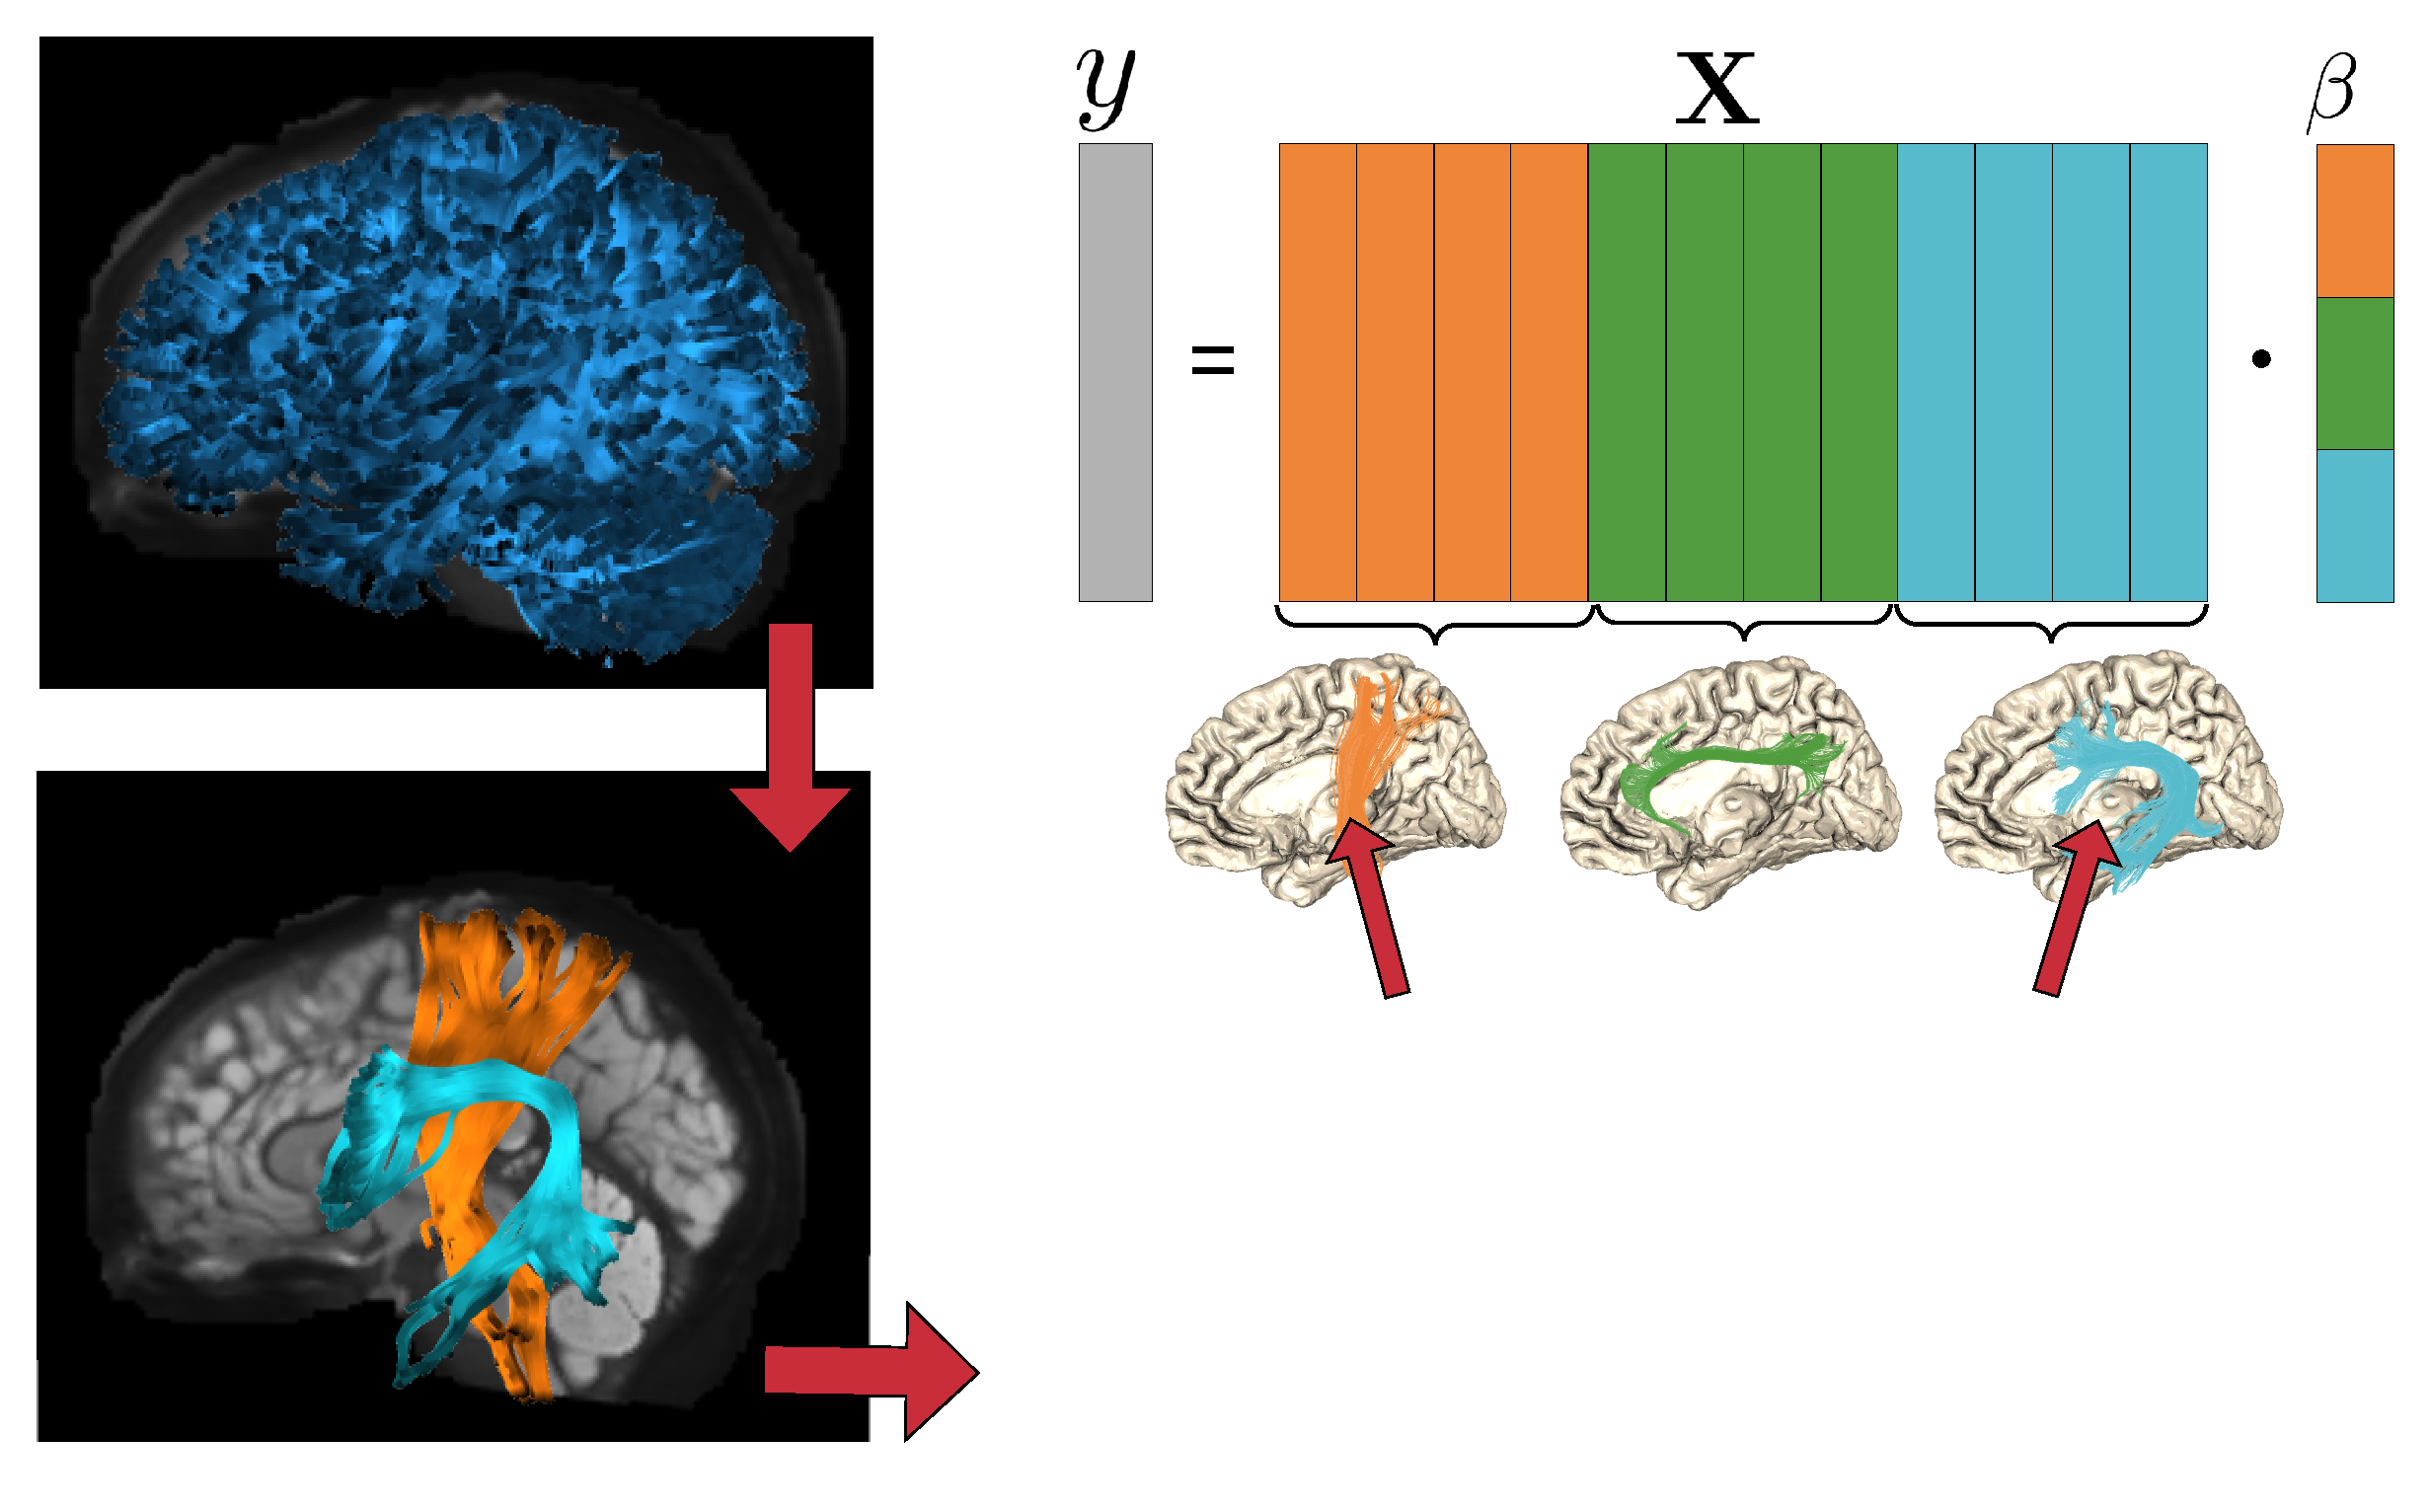
\includegraphics[width=0.98\columnwidth]{methods-brains.pdf}
    }
    \vspace{-8.4cm}
    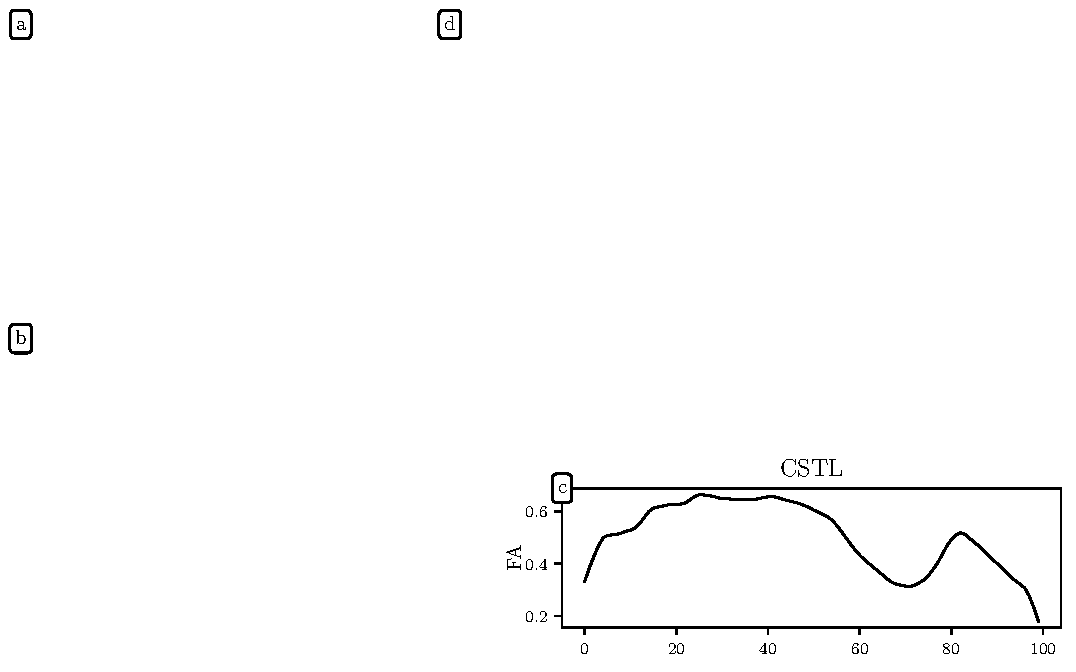
\includegraphics[width=\columnwidth]{method-quad.pdf}
    {\phantomsubcaption\label{fig:methods:tractogram}}
    {\phantomsubcaption\label{fig:methods:cst}}
    {\phantomsubcaption\label{fig:methods:tract-profile:cst}}
    {\phantomsubcaption\label{fig:methods:tract-profile:fa}}
    {\phantomsubcaption\label{fig:methods:group-structure}}
    \caption{\textbf{Tractometry data flow}
        \label{fig:methods}
        \textbf{(a)} Whole brain tractography generates streamlines approximating
        the trajectories of white matter connections.
        \textbf{(b)} Tractometry classifies these streamlines into anatomical bundles.
        In this case, we show the left corticospinal tract (CSTL)
        \added{and the left arcuate fasciculus (ARCL)}
        over a mid-saggital anatomical slice.
        \deleted{\textbf{(c)}} \replaced{Tract profiling}{Tractometry} further extracts bundle profiles,
        quantifications of various diffusion metrics along the length of the
        fiber bundle. Here, we show one subject's fractional anisotropy (FA)
        profile for \added{\textbf{(c)}} the CSTL \added{and \textbf{(d)} the ARCL}.
        \textbf{(d)} the phenotypical target data and \replaced{tract profile}{tractometric}
        features can be organized into a linear model, $\hat{y} = \mathbf{X}
        \hat{\beta}$. The feature matrix $\mathbf{X}$ is color-coded
        to reveal a natural group structure: the left (orange) group
        contains $k$ features from the CSTL, the middle (green) group
        contains $k$ features from the left cingulum cingulate (CGCL),
        and the right (blue) group
        contains $k$ features from the \replaced{ARCL}{left arcuate (ARCL)}.
        The coefficients in $\hat{\beta}$ follow the same natural grouping.
    }
\end{figure}

The present work aims to balance predictive accuracy with descriptive power
\cite{Murdoch2019-ax, Breiman2001-uz} by capitalizing on all of the available
data across all bundles, while also retaining and elucidating spatial
information about the locations that are most informative for discriminative
performance.
\added{Unlike many previous analyses of white matter (e.g., using TBSS \cite{smith2006tract} and connectometry \cite{yeh2016connectometry}), which focus on classical inference about the differences between groups or individuals in terms of their white matter properties, the focus of the present work is on the combination of features that facilitate accurate prediction of the individual differences in a particular phenotype}.
\added{For example, an accurate prediction of which individuals in a group have a particular disease, or a prediction of their age with small error. The distinct goals of \emph{inference} and \emph{prediction} are not necessarily incongruent, but can sometimes be in tension \cite{Bzdok2020-sd}. This distinction is also similar to the distinction between ``encoding'' and ``decoding'' used in the functional MRI literature \cite{Naselaris2011-ss}. In the present work}, we predict the phenotypical variance in a group of subjects,or classify group membership, based on a linear combination of the features estimated with \replaced{tract profiling}{tractometry}.

% Generally speaking, analysis methods should balance predictive
% accuracy with descriptive power \cite{Murdoch2019-ax, Breiman2001-uz}.
% Accordingly, tractometry analysis should simultaneously capitalize on
% all the data across all tracts to make the best possible prediction,
% while also retaining and elucidating spatial information about the
% locations that are most informative for a prediction. In the present
% work, we developed a novel framework for analysis of tractometry that
% simultaneously selects the features for analysis, and fits a model
% to these features. We use a linear modeling approach, which aims to
% predict phenotypical variance in a group of subjects, based on a linear
% combination of the features estimated with tractometry.

Using this approach, we first need to deal with the large and
asymmetric dimensionality of the data: \replaced{tract profile}{tractometry}
data usually has
many more features (i.e., number of measurements per individual) than
samples (number of subjects), which makes inferences from the data
about phenotypical differences between individuals ill-posed. This
regime is the target of several statistical learning techniques, and
is often solved by various forms of regularization.

% For example, Tikhonov regularization shrinks the solution such that the sum of
% squared contributions from the individual features are minimized
% \cite{Hoerl2000-ij}. Another solution to the problem is provided by
% the
The Lasso algorithm minimizes the sum of the absolute values of
contributions of each feature \cite{Tibshirani1996-qs}. This
tends to shrink to zero the contributions of many of the features,
providing results that are both accurate and interpretable. When
additional structure is available in the organization of the data,
regularization algorithms can take advantage of this structure. For
example, if the features lend themselves to a natural division into
different groups, the Group Lasso (GL) can be used to select groups
of features, rather than individual features \cite{Yuan2006-ky}.
The Sparse Group Lasso (SGL) elaborates on this idea by providing
control both of group sparsity, as well as overall sparsity of the
solutions \cite{simon2013sgl}. Because the features measured with
tractomery lend themselves to grouping based on the tracts from which
each measurement is taken, GL and SGL provide useful tools
for linear model fitting in problems of this form. Here we, first,
develop an implementation of SGL that is well suited to the analysis of
\replaced{tract profile}{tractometry} data and, second, demonstrate the power and flexibility of
this approach by applying it to both classification
and continuous prediction problems. Our \deleted{tractometry} data flow is
represented in \cref{fig:methods} and explained in further detail in
the methods section.

\added{One more approach to multivariate analysis of neuroimaging data is to perform inference or prediction in a transformed feature space rather then the original diffusion metric feature space. For example, in Lasso PCR, diffusion features can be projected onto a principal components (PC) basis for use in a sparsity constrained model \mbox{\cite{powell2018local, rasero2021integrating}}. While these approaches achieve high predictive performance and may even yield biologically interpretable principal components \mbox{\cite{chamberland2019dimensionality}}, they neglect anatomical grouping information. We view these approaches as complementary to the SGL-based approach: PCR based approaches seeks to model brain-phenotype relationships using the most parsimonious representation of variance in the diffusion measures. In contrast, our SGL-based approach seeks to establish whether prior knowledge of anatomical grouping improves modeling of brain-phenotype relationships. Motivated by this distinction, we also introduce a union of the two approaches called PCR-SGL, in which each group of features is independently transformed into its PC basis, thereby retaining the anatomical grouping information of the original feature space. We demonstrate circumstances in which this approach both helps and hinders predictive performance.}

% Results
\section*{Results}

We developed a method for analyzing dMRI \replaced{tract profile}{tractometry} data that uses the Sparse
Group Lasso (SGL) to select features that are sparse both at the group (bundle) level, as well as overall.
We demonstrate the use of this method on four different datasets in
both a classification setting and a regression setting.

\subsection*{SGL accurately detects ALS from tractometry data}

Using data from a previous study of patients with amyotrophic lateral sclerosis (ALS)~\cite{sarica2017corticospinal}, we tested the performance of SGL in a
classification setting. The previous study predicted ALS status with a mean
accuracy of 80\% using a random forest algorithm based on \emph{a priori}
selection of features only within the CST bundle-of-interest.
SGL delivers improved predictive performance, with a cross-validated accuracy
of {\alsAccuracy}\% and an area under the receiver operating characteristic
curve (ROC AUC) of {\alsRocAuc}, without the need for \emph{a priori} feature
engineering.
\added{We also predicted ALS diagnosis using the PCR-SGL, wherein each group of features is independently transformed to its PC basis and an SGL model is fit to the transformed features. This model achieves \protect{\alsAccuracyGpca}\% accuracy and an ROC AUC of \protect{\alsRocAucGpca}}
(\cref{fig:class-results:probs}). In addition to this classification
performance, both SGL \added{and PCR-SGL} also \replaced{identify}{identifies}
the white matter tracts most important for ALS classification.
\added{\Cref{fig:class-results:coefs3d} shows that PCR-SGL identified as potential disease biomarkers the diffusion measures in the CST from the cerebral peduncle to the corona radiata, agreeing with the previous study from which these data were extracted \mbox{\cite{sarica2017corticospinal}}.}
The relative importance of white matter
features is captured in the $\beta$ coefficients from \cref{eq:sgl}.
\Cref{fig:class-results:tract-profiles} depicts these coefficients along the
right CST, plotted over the FA values for the control and ALS subject groups \added{(see supplemental Figs S1 and S2 for tract profiles of all 18 tracts in these groups)}.
We find that SGL \replaced{and PCR-SGL select}{selects} FA metrics in the corticospinal tract and
particularly in the right corticospinal tract as most important to ALS
classification, confirming previous findings \cite{van2011upper,
toosy2003diffusion, sarica2014tractography, sage2007quantitative,
sage2009quantitative, karlsborg2004corticospinal, ellis1999diffusion,
cosottini2005diffusion, ciccarelli2009investigation, abe2010voxel} and
identifying the portions of the brain that were selected \emph{a priori} in
the previous study from which we obtained the data
\cite{sarica2017corticospinal}.

\begin{figure}[t!]
    \vspace{3.0cm}
    \rlap{
        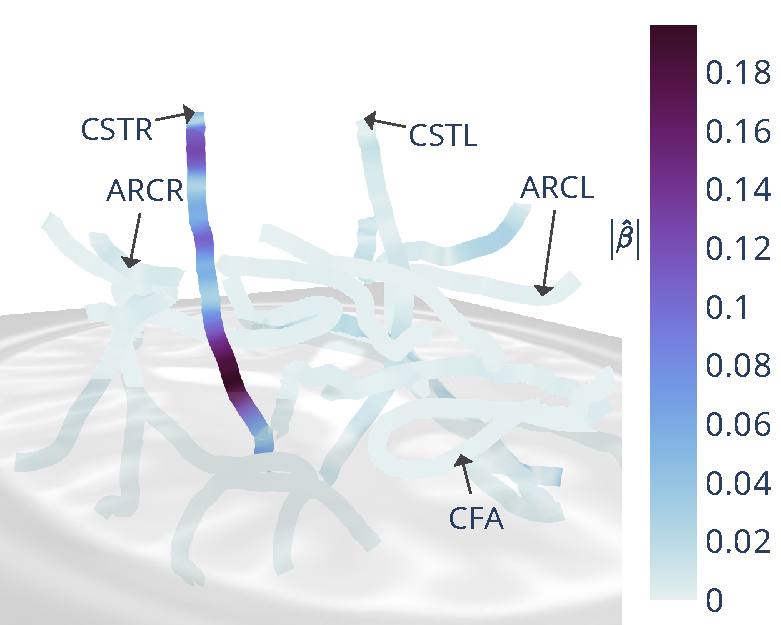
\includegraphics[width=0.33\textwidth]{als_gpca_coefs.pdf}
    }
    \vspace{-7.0cm}
    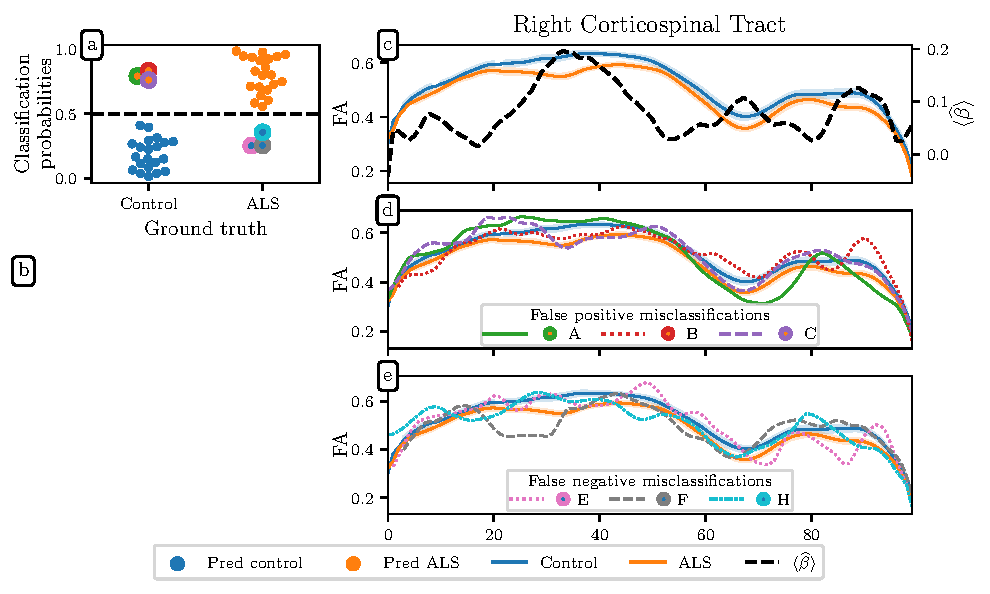
\includegraphics[width=\textwidth]{als_gpca_results.pdf}
    {\phantomsubcaption\label{fig:class-results:probs}}
    {\phantomsubcaption\label{fig:class-results:coefs3d}}
    {\phantomsubcaption\label{fig:class-results:tract-profiles}}
    {\phantomsubcaption\label{fig:class-results:false-positives}}
    {\phantomsubcaption\label{fig:class-results:false-negatives}}
    \caption{%
        {\bf \added{PCR-}SGL accurately and interpretably predicts ALS diagnosis.}
        \label{fig:class-results}
        {\bf (a)} Classification probabilities for ALS diagnosis, with
        controls on the left, patients on the right, predicted controls in
        blue, and predicted patients in orange. That is, orange dots on the left
        represent false positives, while blue dots on the right represent
        false negatives. We achieve {\protect\alsAccuracy}\% accuracy with an
        ROC AUC of {\protect\alsRocAuc}.
        {\bf (b)} \added{PCR-}SGL coefficients are presented on the core fibers of major
        fiber bundles. They exhibit high group sparsity and are concentrated
        in the FA of the \replaced{corticospinal tract (CST)}{CST}.
        The brain is oriented with the right hemisphere
        in the foreground and anterior to the right of the page. The CSTL, CSTR,
        \replaced{callosum forceps anterior (CFA), left arcuate (ARCL), and right arcuate (ARCR)}{CFA}
        bundles are indicated for orientation.
        {\bf (c)} \added{PCR-}SGL identifies three portions of the CST as important,
        where $\hat{\beta}$ (dashed line, right axis) has large values. These
        are centered around nodes 30, 65, and 90, corresponding to locations
        of substantial differences in FA between the ALS and control groups
        (shaded areas indicates standard error of the mean).
        {\bf (d)} Bundle profiles for false positive classifications. Line
        colors correspond to the marker edge color in the top left plot.
        These individuals have reduced FA in the CST portions which SGL
        identified as important. Their misclassification is coherent with the
        feature importance and the group differences in FA.
        {\bf (e)} Individual bundle profiles for false negative
        classifications. These individuals have bundle profiles which
        oscillate between the group means.
    }
\end{figure}

To assess the added value of incorporating anatomical knowledge into our
model, we compared our classification results to those obtained from
\replaced{four other models: a pure lasso model, an elastic net model, a bundle-mean lasso (i.e. a lasso model trained only on the mean metric values from each bundle), and a principal components regression lasso (Lasso PCR) model \cite{powell2018local, rasero2021integrating}}{a lasso model}.
\replaced{These models achieved accuracies of 76\%, 76\%, 79.5\%, and 71.5\% respectively and ROC AUC values of 0.76, 0.75, 0.82, and 0.71, respectively}{The pure lasso model achieved 76\% accuracy and an ROC AUC of 0.76}
using the same cross-validation strategy used to assess the SGL model.
This difference in performance justifies the additional complexity of the SGL
over simpler sparsity-inducing regression strategies.
\added{The relatively poor performance of Lasso PCR suggests that features with small variance are nonetheless relevant for predicting ALS diagnosis. Or equivalently, that group differences between ALS diagnoses are not the dominant source of variance in the diffusion metrics.}

The $\beta$ coefficients exhibit high bundle level sparsity; only some
bundles are important, which can be be confirmed by observing the value of
$\alpha$, the regularization hyperparameter that controls the mixture of the
Group Lasso and lasso penalties, selected through nested cross-validation
(see \cref{eq:sgl}).
If $\alpha$ is closer to zero, it indicates that the phenotype in question
preferentially correlates with only a few groups of covariates. For the ALS
dataset, \added{the SGL model has} $\alpha = $ \alsLRatio
~\added{and the PCR-SGL model has \protect$\alpha = $ \protect\alsLRatioGpca},
confirming that the white matter correlates of ALS reside mostly in one
bundle, namely the CST.

Analyzing the ways in which the model mislabels individuals also provides
insight. We found that mislabelled subjects are outliers relative to their
group with respect to diffusion features of the CST
(\cref{fig:class-results:false-positives,fig:class-results:false-negatives}).
The false positive classifications have reduced FA in one or more of the
three sections of the CST where $\norm*{\hat{\beta}}$ is large in
\cref{fig:class-results:tract-profiles}. The false negative subjects have FA
profiles that oscillate between the two group means. Thus, when the SGL
method predicts incorrectly this is done in a comprehensible manner.

\subsection*{SGL accurately predicts age from tractometry data}

To test the performance of SGL \deleted{with tractometry data} in a continuous
regression task, we focus here on the prediction of biological age in three
datasets named WH, HBN, and Cam-CAN (see the Methods section for a description of each dataset). Prediction of ``brain
age'' is a commonly undertaken task in neuroimaging machine learning, in part
because these predictions, and deviations therefrom, may be diagnostic of
overall brain health (for a review, see Cole et al.~\cite{Cole2019-rz}).
However, as Nelson et al.~\cite{nelson2019biomarkers} have observed, aging
biomarkers are subject to unique challenges and tend to be noncausative. Our
interest in aging here relies on its utility as a methodological benchmark.
Biological age operates on a natural scale, with meaningful and easily
understood units, and it's popularity as a machine learning target makes it
valuable for comparisons with other studies.

The WH \cite{yeatman2014lifespan}, HBN \cite{alexander2017open}, and Cam-CAN
\cite{shafto2014cambridge,taylor2017cambridge} datasets used here contain
data from 76, 1651, and 640 subjects, respectively, ranging from 6-50, 5-21,
and 18-88 years of age, respectively. In each case, biological age was used
as the predicted variable $y$. SGL was fit to the \replaced{tract profile}{tractometry-extracted}
features FA and mean diffusivity (MD) in 18 major brain tracts, with diffusion metrics extracted
from diffusion tensor imaging (DTI) for the WH dataset and diffusion kurtosis
imaging (DKI) \cite{jensen2005diffusion} for the HBN and Cam-CAN datasets \added{see supplemental Figs S3 to S8 for the full tract profile information in all tracts/datasets}.

\begin{figure}[t!]
    \vspace{3.0cm}
    \rlap{
        \hspace{0.775cm}
        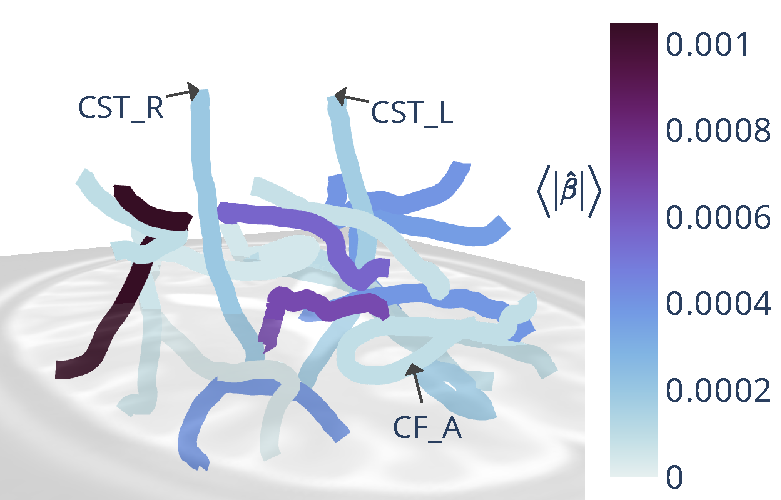
\includegraphics[width=0.26\textwidth]{wh_coefs.pdf}
        \hspace{0.5em}
        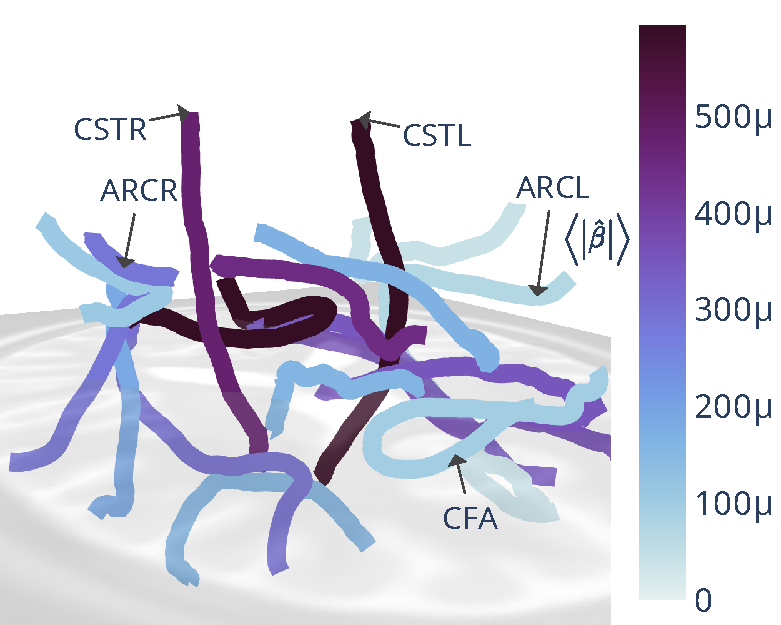
\includegraphics[width=0.26\textwidth]{hbn_coefs.pdf}
        \hspace{0.5em}
        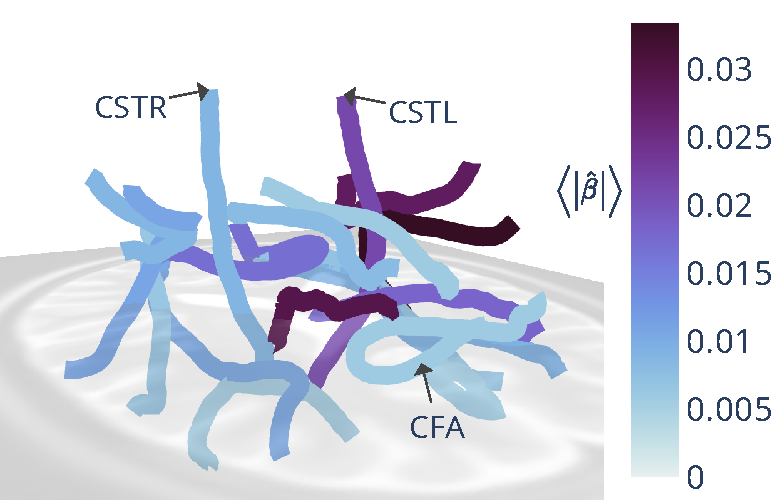
\includegraphics[width=0.26\textwidth]{camcan_coefs.pdf}
    }
    \vspace{-6.1cm}
    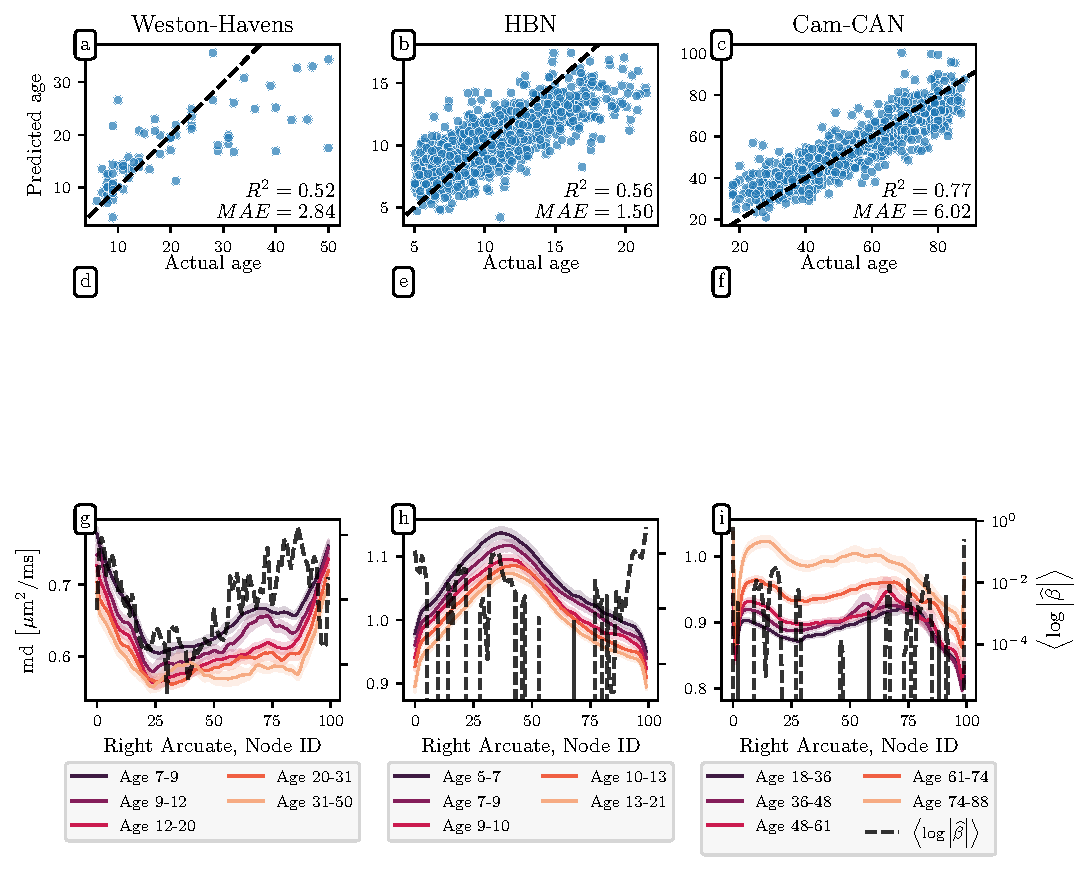
\includegraphics[width=\textwidth]{regression_scatter.pdf}
    {\phantomsubcaption\label{fig:age-results:wh-scatter}}
    {\phantomsubcaption\label{fig:age-results:hbn-scatter}}
    {\phantomsubcaption\label{fig:age-results:cc-scatter}}
    {\phantomsubcaption\label{fig:age-results:wh-coefs3d}}
    {\phantomsubcaption\label{fig:age-results:hbn-coefs3d}}
    {\phantomsubcaption\label{fig:age-results:cc-coefs3d}}
    {\phantomsubcaption\label{fig:age-results:wh-profile}}
    {\phantomsubcaption\label{fig:age-results:hbn-profile}}
    {\phantomsubcaption\label{fig:age-results:cc-profile}}
    \caption{%
        {\bf Predicting age with tractometry and SGL.}
        \label{fig:age-results}
        {\bf (top)} The predicted age vs. true age of each individual from the test
        splits (i.e., when each subject's data was held out in fitting the
        model) for the {\bf (a)} WH, {\bf (b)} HBN, and {\bf (c)} Cam-CAN
        datasets; an accurate prediction falls close to the $y=x$ line
        (dashed). The mean absolute error (MAE) and coefficient of
        determination $R^2$ are presented in the lower right of each scatter
        plot.
        {\bf (middle)} Feature importance for predicting age from
        \replaced{tract profile}{tractometry} in
        the {\bf (d)} WH, {\bf (e)} HBN, and {\bf (f)} Cam-CAN datasets.
        The orientation of the
        brain is that same as in \cref{fig:class-results:coefs3d}, however because
        the coefficients exhibit high global sparsity (as opposed to group
        sparsity), we plot the mean of the absolute value of $\hat{\beta}$
        for each bundle on the core fiber. The global distrubution of the
        $\hat{\beta}$ coefficients reflects the fact that aging is not
        confined to a single white matter bundle.
        {\bf (bottom)} Age quintile bundle profiles for the {\bf (g)} WH,
        {\bf (h)} HBN, and {\bf (i)} Cam-CAN datasets.
    }
\end{figure}

To evaluate the fit of the model, we used a nested cross-validation
procedure. In this procedure, batches of subjects are held out. For each
batch (or fold), the model is fully fit without this data. Then, once the
parameters are fixed, the model is applied to predict the ages of held out
subjects based on the linear coeffiecients. This scheme automatically finds
the right level of sparsity and fits the coefficients to the ill-posed linear
model, while guarding against overfitting. SGL accurately predicts the age of
the subjects in this procedure, with a median absolute error of {\whMae},
\added{{\hbnMae}}, and {\camcanMae} years for the WH, HBN, and Cam-CAN datasets,
respectively and coefficients of determination $R^2 = $ {\whRsq} , \added{{\hbnRsq}}, and {\camcanRsq},
respectively (see \cref{fig:age-results}, top panels). The
predictions for Cam-CAN are competitive with a recent state of the art
prediction \cite{mcpherson2020single}, which used streamline density to
estimate the brain's structural connectivity and achieved $R^2 = 0.63$. The
median absolute errors are also lower than the results of a recent study that
predicted age in a large sample that included the Cam-CAN data, and was based
on diffusion MRI features \cite{Richard2018-ux}.

In contrast to the ALS classification case, the selected $\alpha$ values
indicate high global sparsity over group sparsity, with $\alpha = $
{\whLRatio}, {\hbnLRatio}, and {\ccLRatio}, for the WH, HBN, and Cam-CAN
datasets, respectively. The model weights are distributed over many different
tracts and dMRI tissue properties (see
\cref{fig:age-results:wh-coefs3d,fig:age-results:hbn-coefs3d,fig:age-results:cc-coefs3d}
and supporing figures in \nameref{S1_Appendix}).
This demonstrates that SGL is not coerced to produce overly sparse results
when a more accurate model requires a dense selection of features.
Furthermore, inspecting the portions of bundles with larger coefficients in
\cref{fig:age-results:wh-profile,fig:age-results:hbn-profile,fig:age-results:cc-profile}
reveals that SGL selects informative regions where diffusion properties are
different between the age quintiles.

As with ALS classification, we also compared SGL performance with results
obtained using
\replaced{the pure lasso, elastic net, bundle-mean lasso, and Lasso PCR}{only the lasso penalty}.
The pure lasso models achieved $R^2 = 0.47$, $0.54$, and $0.70$ for the WH, HBN, and Cam-CAN datasets respectively using the same cross-validation strategy used to assess the SGL.
\added{The elastic net models achieved $R^2 = 0.46$, $0.59$, and $0.73$ for the WH, HBN, and Cam-CAN datasets, respectively. The bundle-mean lasso models achieved $R^2 = 0.33$, $0.22$, and $0.55$, respectively. And the Lasso PCR models achieved $R^2 = 0.54$, $0.57$, $0.74$, respectively.}
The SGL models'
performance improvement over lasso is more modest than in the ALS
classification case, which accords with the selected values of the $\alpha$
hyperparameter. These SGL models were more lasso-like in their sparsity
penalties so they are more lasso-like in their predictive performance.

\begin{figure}[t!]
    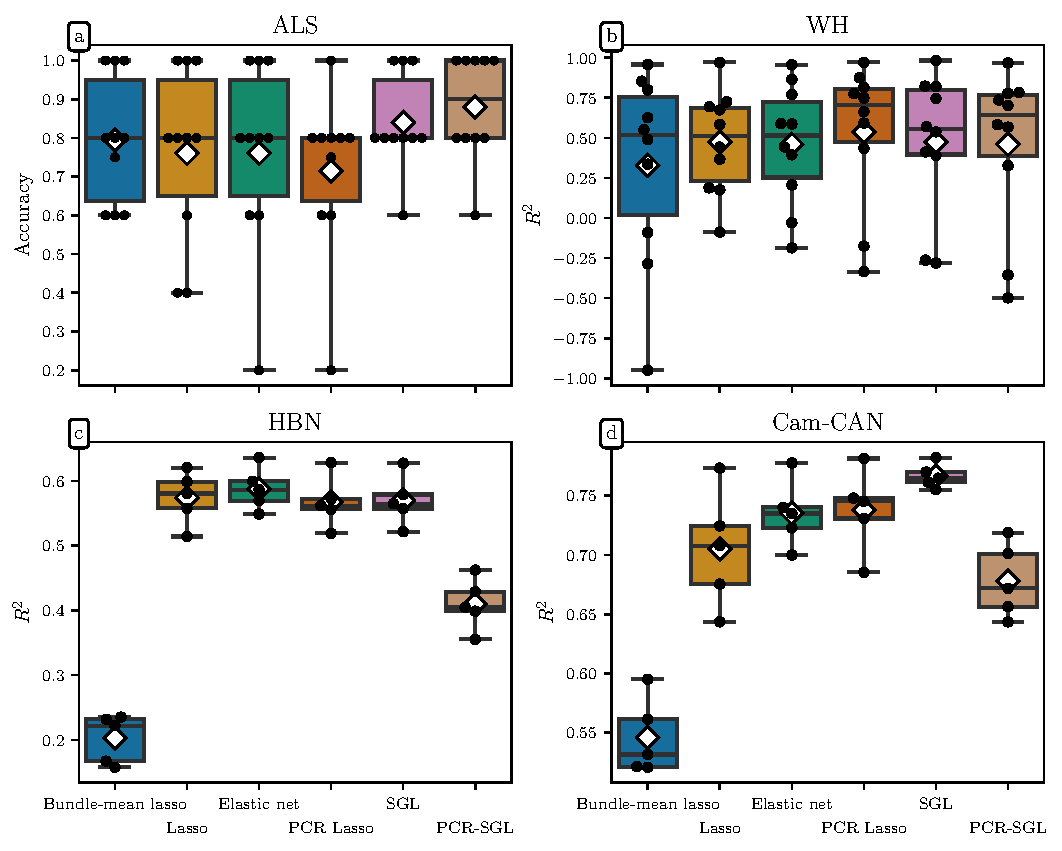
\includegraphics[width=\textwidth]{model_performance.pdf}
    \caption{%
        {\bf \added{Model performance across all datasets.}}
        \label{fig:model-performance}
        \added{Each panel shows model performance measured on the test set for each}
        \added{cross-validation split, with each black dot representing a split, box}
        \added{plots representing the quartiles, and white diamonds representing the mean}
        \added{performance. The $y$-scale varies in each subplot.}
        \added{\textbf{(a)} Accuracy of test set predictions for the}
        \added{ALS dataset. Because group differences}
        \added{in ALS diagnosis are mostly confined to a single bundle, the group}
        \added{structure-preserving methods, SGL and PCR-SGL, outperform the other}
        \added{models.}
        \added{The remaining frames show coefficient of determination, \protect$R^2$ in test sets}
        \added{for the \textbf{(b)} WH, \textbf{(c)} HBN, and \textbf{(c)} Cam-CAN}
        \added{datasets. Because aging affects the white matter globally, group structure-blind}
        \added{methods like elastic net and PCR Lasso perform well. Nonetheless, the SGL}
        \added{models show competitve predictive performance, adapting to a problem where}
        \added{group structure is not as informative. PCR-SGL performs poorly in this regime}
        \added{because its initial group-wise PC projection destroys between bundle covariance.}
        \added{The bundle-mean lasso performs poorly, demonstrating the value of along-tract profiling.}
    }
\end{figure}
\added{Model performance across all four datasets and all six model types is summarized}
\added{in \cref{fig:model-performance}. In contrast to the ALS classification case, the PCR Lasso performs}
\added{competitively in age regression, suggesting that aging is a significant source of global variance}
\added{in the tract profiles. On the other hand, the PCR-SGL models destroy cross-bundle covariance information}
\added{in their initial group-wise PC projection step (see \cref{eq:svd}), limiting performance}
\added{for globally distributed phenomena. Conversely, the SGL models are able to adapt to this regime.}

\section*{Discussion}

We present here a novel method for analysis of dMRI \replaced{tract profile}{tractometry} data that
relies on the Sparse Group Lasso \cite{simon2013sparse} to make accurate
predictions of phenotypic properties of individual subjects while,
simultaneously, identifying the features of the white matter that are most
important for this prediction. The method is data-driven and it is broadly
applicable to a wide range of research questions: it performs well in
predicting both continuous variables, such as biological age, as well as
categorical variables, such as whether a person is a patient or a healthy
control. In both of these cases, SGL out-performs previous algorithms that
have been developed for these tasks \cite{sarica2017corticospinal,
Richard2018-ux, mcpherson2020single}. The nested cross-validation approach
used to fit the model and make both predictions and inferences from the model
guards against overfitting and tunes the degree of sparseness required by the
algorithm. This means that SGL can accurately describe phenomena that are
locally confined to a particular anatomical location or diffusion property
(e.g., FA in the CST) as well as phenomena that are widely distributed
amongst brain regions and measured diffusion properties.

Specifically, we demonstrated that the algorithm correctly detects the fact
that ALS, which is a disease of lower motor neurons, is localized to the
cortico-spinal tract. This recapitulates the results of previous analysis of
these same data, using a bundle-of-interest approach
\cite{sarica2017corticospinal}.
\added{As with the original study, it is unclear whether our strong predictive performance based on image properties that would be visible in patient scans or whether it is identifying a new subclinical disease biomarker.}
In contrast, for the analysis of biological
age, the coefficients identified by the algorithm are very widely distributed
across many parts of the white matter, mirroring previous results that show a
large and continuous distribution of life-span changes in white matter
properties \cite{yeatman2014lifespan}.
\added{We present age quintile bundle profiles and SGL \protect$\beta$ coefficients for all four datasets in the supplementary material. For age regression, substantial differences between the datasets preclude generalization across all three:}
\begin{enumerate*}[%
    label=(\roman*),%
    before=\unskip{: },%
    itemjoin={{, }},%
    itemjoin*={{, and }}]
    \item \added{different acquisition parameters, which can be challenging to harmonize \mbox{\cite{pinto2020harmonization}}}
    \item \added{different diffusion models, with DTI for the WH dataset and DKI for the HBN and Cam-CAN datasets}
    \item \added{different age ranges and distributions (which is evident in the figure legends for \cref{fig:age-results}), with HBN being a developmental dataset, while WH and Cam-CAN are lifespan maturation datasets}
    \item \added{different anatomical extents, with the WH streamlines truncated to remain with the bundle's bounding regions of interest (the default behavior in the legacy \texttt{mAFQ}) and the HBN and Cam-CAN streamlines allowed to retain their full extent from whole-brain tractography (the default behavior in \texttt{pyAFQ}).}
\end{enumerate*}
\added{In a biological characteristic that has widespread effects in the brain, validity is difficult to assess \mbox{\cite{lermausabiaga2019replication}}, so it is both unsurprising and vexing that we can do so well at predicting within each dataset, and yet do poorly in interpreting informative features across instruments.}


\added{We also implemented a union of the PCR Lasso and SGL approaches by first}
\added{projecting each group onto its PC basis. This PCR-SGL approach transformed the feature}
\added{space into a more parsimonious representation of its variance while}
\added{also preserving group structure. But it was unable to efficiently represent}
\added{cross-bundle covariance, which is an advantage of PCR Lasso. As a result, PCR-SGL performed well in ALS classification,}
\added{where the white matter interactions are highly localized, and poorly}
\added{in age regression, where the white matter interactions are global.}

One drawback of our approach is also evident in the age regression results.
There are portions of the bundle profiles in
\cref{fig:age-results:wh-profile,fig:age-results:hbn-profile,fig:age-results:cc-profile}
for which the $\hat{\beta}$ coefficients are zero but for which the bundle
profiles clearly contain an age differentiating signal. While SGL correctly
identifies certain features as important, it is not guaranteed to identify
\emph{all} of the important features. It will identify a parsimonious set of
important features, dense enough to predict the phenotype and sparse enough
(at either the group or global level) to satisfy the sparsity constraints.

\added{Another limitation of our approach is in its computational execution time, which, in our experience, is roughly five times slower than simpler models like the lasso. This slow-down is likely to be insignificant for ``production'' cycles in which researchers report their findings, but may be prohibitive for ``development'' cycles in which researchers repeatedly train models while adjusting their analysis pipeline. In practice, we circumvent this limitation by developing our analysis infrastructure with fast, simple models, and substituting slower, more performant models afterwards. The consistent scikit-learn-based application programming interface of \texttt{AFQ-Insight} provides a good basis for this pattern.}

Taken together, \replaced{our}{these} results demonstrate the promise of the
group-regularized regression approach. Even at the scale of dozens of
subjects, the results provided by SGL are both accurate, as well as
interpretable \cite{Murdoch2019-ax}: \replaced{tract profiling}{tractometry} capitalizes on domain
knowledge to engineer meaningful features; SGL scores these features based on
their relative importance; enables a visualization of these feature
importance scores in the anatomical coordinate frame of the bundles (e.g.,
\cref{fig:class-results:coefs3d,fig:age-results:wh-coefs3d,fig:age-results:hbn-coefs3d,fig:age-results:cc-coefs3d})
and provides a means to understand model errors (e.g.,
\cref{fig:class-results:false-positives,fig:class-results:false-negatives}).
Thus, this multivariate analysis approach achieves high cross-validated
accuracy for precision medicine applications of dMRI data and identifies
relevant features of brain anatomy that can further our neuroscientific
understanding of clinical disorders.

Neuroscience has entered an era in which consortium efforts are amassing
large datasets of high-quality dMRI measurements to address a variety of
scientific questions \cite{jernigan2016ping, jernigan2018abcd,
alexander2017open, Miller2016-hw, VanEssen2012}, but the volume and
complexity of these data pose substantial challenges.
\replaced{Tract profiling}{Tractometry} followed by
analysis with SGL provide a promising approach to distill meaningful insights
from the wealth of data measured in these efforts.

SGL has many other potential applications in neuroscience, because of the
hierarchical and grouped nature of many data types that are collected in
multiple sample points within anatomically-defined areas. For example, this
method may be useful to understand the relationship between fMRI recordings
and behavior, where activity in each voxel may co-vary with voxels within the
same anatomical region and form features and groups of features. Similarly,
large-scale multi-electrode recordings of neural activity in awake behaving
animals are becoming increasingly feasible \cite{steinmetz2018distributed,
Jun2017-gv} and these recordings can form features (neurons) and groups
(neurons within an anatomical region).

% More ambitiously perhaps, this approach may be
% used to understand the role of correlations in so-called resting-state
% fMRI time-series and behavior, where pairwise correlations between
% voxels in different anatomical regions are features in the matrix and
% features may be grouped by pairs of anatomical regions. Given the large
% number of voxels in the surface of the gray matter and given that
% correlations increase the number of features by a factor of $n^2$, this
% would pose a challenging problem to solve using SGL.
The results we present here also motivate extensions of the method using more
sophisticated cost functions. For example, the fused sparse group lasso
(FSGL) \cite{zhou2012} extends SGL to enforce additional spatial structure:
smoothness in the variation of diffusion metrics along the bundles. As brain
measurements include additional structure (for example, bilateral symmetry),
future work could also incorporate overlapping group membership for each
entry in the tract profiles \cite{Rao2014-xm}. For example, a measurement
could come from the corpus callosum, but also from the right hemipshere. This
would also require extending the cost function used here to incorporate these
constraints. Similarly, unsupervised dimensionality reduction of tractometry
data (e.g., \cite{chamberland2019dimensionality}) could also benefit from constraints
based on grouping\added{, as our implementation of PCR-SGL suggests}.

The method is packaged as open-source software called AFQ-Insight that is
openly available at \url{https://github.com/richford/AFQ-Insight}, and
provides a clear API to allow for extensions of the method. The sofware
integrates within a broader automated fiber quantification software
ecosystem: AFQ \cite{yeatman2012tract} and pyAFQ \cite{kruper2021evaluating}, which extract
\replaced{tract profile}{tractometry} data from raw and processed dMRI datasets, as well as
AFQ-Browser, which visualizes \replaced{tract profiles}{tractometry} data and facilitates sharing of the
results of dMRI studies \cite{yeatman2018browser}. To facilitate
reproducibility and ease use of the software, the results presented in this
paper are also provided in
\url{https://github.com/richford/afq-insight-paper} as a series of Jupyter
notebooks \cite{kluyver2016jupyter}.

\section*{Materials and methods}
\label{sec:methods}

\subsection*{Data}
\label{sec:data}

Four different datasets were used here:

\begin{enumerate}

\item Diffusion MRI from a previous study of the corticospinal
tract (CST) in patients with amyotrophic lateral sclerosis
(ALS \cite{sarica2017corticospinal}), containing data from 24 ALS
patients and 24 demographically matched healthy controls. These data
were measured in a GE Discovery 750 3T MRI scanner at the Institute
of Bioimaging and Molecular Physiology in Catanzaro. Informed consent
was provided as approved by the Ethical Committee of the University
``Magna Graecia'' of Catanzaro. Voxel resolution was \num{2x2x2}
$\text{mm}^3$ and 27 non-colinear directions were measured with a
$b=1000$ $\text{s} / \text{mm}^2$. Data was preprocessed to
correct for subject motion and for eddy currents. The diffusion tensor
model \cite{basser1994mr} was fit in every voxel.
We will refer to this dataset as ALS.

\item Diffusion MRI data from a previous study of properties of
the white matter across the lifespan \cite{yeatman2014lifespan},
containing dMRI data from 76 subjects with ages 6-50. These data were
measured in a GE Discovery 750 3T MRI scanner at the Stanford Center
for Cognitive and Neurobiological Imaging. The Stanford University
IRB approved the procedures of this study. Informed consent was
obtained from each adult participant, and assent for participation
was provided by parents/guardians for children. Voxel resolution was
\num{2x2x2}$\textrm{mm}^3$ with 96 non-colinear directions measured with a
$b=2000$ $\textrm{s} / \textrm{mm}^2$ and 30 non-colinear directions
measured with a $b=1000$ $\textrm{s} / \textrm{mm}^2$. These data
were acquired using a dual spin echo sequence, in which there is
sufficient time for eddy currents to subside between the application of
the gradients and the image acquisition, so no eddy current correction
was applied, but motion correction was applied before fitting the
diffusion tensor model \cite{basser1994mr} in every voxel using a robust
fit \cite{chang2005restore}
\added{on the \protect$b=1000$ \protect$\textrm{s} / \textrm{mm}^2$ shell only}.
We will refer to this dataset as WH.

\item Diffusion MRI data from the Healthy Brain Network pediatric mental
health study \cite{alexander2017open}, containing dMRI data from 1651 subjects
with ages 5-21. These data were measured in 3T Siemens MRI scanners at two
sites in the New York
area\added{: Rutgers University Brain Imaging Center and the CitiGroup Cornell Brain Imaging Center}.
Informed consent was obtained from each participant aged 18 or older. For
participants younger than 18, written consent was obtained from their legal
guardians and written assent was obtained from the participant. Voxel
resolution was \num{1.8x1.8x1.8}$\text{mm}^3$ with 64 non-colinear directions
measured for each of $b=1000 \text{s} / \text{mm}^2$ and $b=2000 \text{s} /
\text{mm}^2$. Preprocessing was performed using \emph{QSIPrep} 0.12.1, which
is based on \emph{Nipype} 1.5.1 \cite[RRID:SCR\_002502]{nipype1,nipype2}.

\begin{itemize}

\item {\it Anatomical data preprocessing}
The T1-weighted (T1w) image was corrected for intensity non-uniformity
(INU) using \texttt{N4BiasFieldCorrection} \cite[ANTs 2.3.1]{n4}, and
used as T1w-reference throughout the workflow. The T1w-reference was
then skull-stripped using \texttt{antsBrainExtraction.sh} (ANTs 2.3.1),
using OASIS as target template. Spatial normalization to the ICBM 152
Nonlinear Asymmetrical template version 2009c
\cite[RRID:SCR\_008796]{mni} was performed through nonlinear
registration with \texttt{antsRegistration} \cite[ANTs 2.3.1,
RRID:SCR\_004757]{ants}, using brain-extracted versions of both T1w
volume and template. Brain tissue segmentation of cerebrospinal fluid
(CSF), white-matter (WM) and gray-matter (GM) was performed on the
brain-extracted T1w using \texttt{FAST} \cite[FSL 6.0.3:b862cdd5,
RRID:SCR\_002823]{fsl_fast}.

\item {\it Diffusion data preprocessing}

Any images with a b-value less than 100 s/mm\^{}2 were treated as a
\emph{b}=0 image. MP-PCA denoising as implemented in MRtrix3's
\texttt{dwidenoise}\cite{dwidenoise1} was applied with a 5-voxel
window. After MP-PCA, B1 field inhomogeneity was corrected using
\texttt{dwibiascorrect} from MRtrix3 with the N4 algorithm \cite{n4}.
After B1 bias correction, the mean intensity of the DWI series was
adjusted so all the mean intensity of the b=0 images matched across
eachseparate DWI scanning sequence.

FSL (version 6.0.3:b862cdd5)'s eddy was used for head motion correction
and Eddy current correction \cite{anderssoneddy}. Eddy was configured
with a \(q\)-space smoothing factor of 10, a total of 5 iterations, and
1000 voxels used to estimate hyperparameters. A linear first level model
and a linear second level model were used to characterize Eddy
current-related spatial distortion. \(q\)-space coordinates were
forcefully assigned to shells. Field offset was attempted to be
separated from subject movement. Shells were aligned post-eddy. Eddy's
outlier replacement was run \cite{eddyrepol}. Data were grouped by
slice, only including values from slices determined to contain at least
250 intracerebral voxels. Groups deviating by more than 4 standard
deviations from the prediction had their data replaced with imputed
values. Data was collected with reversed phase-encode blips, resulting
in pairs of images with distortions going in opposite directions. Here,
b=0 reference images with reversed phase encoding directions were used
along with an equal number of b=0 images extracted from the DWI scans.
From these pairs the susceptibility-induced off-resonance field was
estimated using a method similar to that described in \cite{topup}. The
fieldmaps were ultimately incorporated into the Eddy current and head
motion correction interpolation. Final interpolation was performed using
the \texttt{jac} method.

Several confounding time-series were calculated based on the
\emph{preprocessed DWI}: framewise displacement (FD) using the implementation
in \emph{Nipype} following the definitions by \cite{power_fd_dvars}. The DWI
time-series were resampled to ACPC, generating a \emph{preprocessed DWI run
in ACPC space}.

\item \added{{\it MRtrix3 Reconstruction}}

\added{Reconstruction was performed using \emph{QSIprep} 0.12.1. Multi-tissue fiber response functions were estimated using the dhollander algorithm. FODs were estimated via constrained spherical deconvolution (CSD, \mbox{\cite{originalcsd, tournier2008csd}}) using an unsupervised multi-tissue method \mbox{\cite{dhollander2019response, dhollander2016unsupervised}}. Reconstruction was done using MRtrix3 \mbox{\cite{mrtrix3}}. FODs were intensity-normalized using mtnormalize \mbox{\cite{mtnormalize}}.}
\end{itemize}

Many internal operations of \emph{QSIPrep} use \emph{Nilearn} 0.6.2
\cite[RRID:SCR\_001362]{nilearn} and \emph{DIPY} \cite{dipy}. For more
details of the pipeline, see
\href{https://qsiprep.readthedocs.io/en/latest/workflows.html}{the
section corresponding to workflows in \emph{QSIPrep}'s documentation}.
We will refer to this dataset as HBN.

\item Diffusion MRI data from the Cambridge Centre for Ageing and
Neuroscience (Cam-CAN) ``CC700'' dataset
\cite{shafto2014cambridge,taylor2017cambridge}, containing data from 640
subjects with ages 18-88. These data were measured on a 3T Siemens TIM Trio
system and written informed consent was obtained from each participant. Voxel
resolution was \num{2x2x2}$\text{mm}^3$ with 30 non-colinear directions
measured for each of $b=1000$ $\text{s} / \text{mm}^2$ and $b=2000$
$\text{s} / \text{mm}^2$. The diffusion weighted images were acquired
with a twice refocused spin-echo sequence and the same preprocessing
\replaced{and reconstruction pipelines}{pipeline}
used for the HBN dataset was applied to this data. We will refer to this
dataset as Cam-CAN.

\end{enumerate}

Data from the ALS and WH studies was processed in a similar manner,
using the Matlab Automated Fiber Quantification toolbox
(\texttt{mAFQ}\added{, version 1.1 for WH and version 1.2 for ALS})
\cite{yeatman2012tract}: streamlines representing fascicles of white
matter tracts were generated using a determinstic tractography algorithm
that follows the prinicpal diffusion direction of the diffusion tensor
in each voxel (STT) \cite{basser2000vivo}. \replaced{Eighteen major}{Major}
tracts\added{, which are enumerated in the supplemental material,} were identified
using multiple criteria: streamlines are selected as candidates for
inclusion in a bundle of streamlines that represents a tract if they
pass through known inclusion ROIs and do not pass through exclusion
ROIs \cite{wakana2007reproducibility}. In addition, a probabilistic
atlas is used to exclude streamlines which are unlikely to be part of
a tract \cite{Hua2008-sh}. Each streamline is resampled to 100 nodes
and the robust mean at each location is calculated by estimating the 3D
covariance of the location of each node and excluding streamlines that
are more than 5 standard deviations from the mean location in any node.
Finally, a bundle profile of tissue properties in each bundle was created
by interpolating the value of MRI maps of these tissue properties to the
location of the nodes of the resampled streamlines designated to each
bundle. In each of 100 nodes, the values are summed across streamlines,
weighting the contribution of each streamline by the inverse of the
\replaced{mahalanobis}{mahalnobis} distance of the node from the average of
that node across streamlines. This means that streamlines that are more
representative of the tract contribute more to the bundle profile, relative
to streamlines that are on the edge of the tract.

Data from the HBN and Cam-CAN studies were processed using the updated Python
Automated Fiber Quantification toolbox (\texttt{pyAFQ}; \cite{kruper2021evaluating}). In
addition to demonstrating the our analysis pipeline is robust to changes in
tractometry software, the use of the updated \texttt{pyAFQ} capitalized upon
the following improvements over the legacy Matlab version
\begin{enumerate*}[%
    label=(\roman*),%
    before=\unskip{: },%
    itemjoin={{, }},%
    itemjoin*={{, and }}]
    \item the ability to ingest data provided in the BIDS format
    \cite{gorgolewski2016brain}
    \item the calculation of diffusion kurtosis imaging (DKI
    \cite{jensen2005diffusion}) metrics
\end{enumerate*}
We will refer to the \texttt{mAFQ} and \texttt{pyAFQ} pipeline collectively
as \texttt{AFQ}.

These processes create bundle profiles, in which diffusion measures
are quantified and averaged along eighteen major fiber tracts,
which are enumerated in the supplemental material.
\added{See Fig S3 of \mbox{\cite{kruper2021evaluating}} for a depiction of these white matter bundles.}
Here,
we use only the mean diffusivity (MD) and the fractional anisotropy
(FA) of the diffusion tensor, but additional dMRI-based maps or maps
based on other quantitative MRI measurements can also be used.
\added{The resulting feature space was the same for all four datasets, with the FA and MD metrics at each of 100 nodes in eighteen bundles comprising 3600 features per subject.}
These bundle profiles, along with the phenotypical data we wish to explain
or predict, form the input to the SGL algorithm. In a domain-agnostic
machine learning context, the phenotypical data comprise the target
variables while the bundle profiles form the feature or predictor
variables (\replaced{see}{See} \cref{fig:methods:group-structure}).

\subsubsection*{\added{Data harmonization for HBN}}

\added{For the multisite HBN study, we use the ComBat harmonization method to robustly adjust for site effects in the tract profiles. Initially designed to correct for site effects in gene expression studies \mbox{\cite{johnson2007adjusting}}, ComBat employs a parametric empirical Bayes approach to adjust for batch effects and has since been applied to multi-site cortical thickness measurements \mbox{\cite{fortin2018harmonization}}, multi-site DTI studies \mbox{\cite{fortin2017harmonization}}, and functional MRI data in the Adolescent Brain Cognitive Development Study (ABCD) \mbox{\cite{nielson2018detecting}}. We rely on the \texttt{neurocombat\_sklearn} library \mbox{\cite{neurocombat_sklearn}}, to apply ComBat in our scikit-learn analysis pipeline and present bundle profile site differences in the supplemental material.}

\subsection*{Sparse Group Lasso}
\label{sec:sgl}

Before fitting a model to the data, imputation and standardization are
performed. Missing node values (e.g., in cases where \texttt{AFQ} designates
a node as not-a-number) are imputed via linear interpolation. Care is taken
not to interpolate across the boundaries between different bundles. Some
diffusion metrics will have naturally larger variance than others and may
therefore dominate the objective function and make the SGL estimator unable
to learn from the lower variance metrics. For example, fractional anisotropy
(FA) is bounded between zero and one and could be overwhelmed by an unscaled
higher-variance metric like the mean diffusivity (MD). To prevent this we
remove each feature's mean and scale it to unit variance (z-score) using the
\lstinline|StandardScaler| from scikit-learn \cite{scikit-learn}. The scaling
parameters are learned only from the training data and then applied equally
to the training and test data in order to prevent leakage of information
between the testing and training sets \cite{kaufman2012leakage}.

After scaling and imputation, the \replaced{tract profile}{tractometry} data and target
phenotypical data can be organized in a linear model:
\begin{equation}
    y = \mathbf{X} \beta + \epsilon,
    \label{eq:lm}
\end{equation}
where $y$ is the phenotype -- categorical, such as a clinical diagnosis,
or continuous numerical, such as the subject's age. The \replaced{tract profile}{tractometry}
data is represented in the feature matrix $\mathbf{X}$, with rows
corresponding to different subjects, and columns corresponding
to diffusion measures at different nodes within each bundle. The
relationship between tractometric features and the phenotypic target is
characterized by the coefficients in $\beta$. The error term, $\epsilon$
is an unobserved random variable that captures the error in the model.
We denote our prediction of the target phenotype as $\hat{y}$ and the
coefficients that produce this prediction as $\hat{\beta}$, so that
\begin{equation}
    \hat{y} = \mathbf{X} \hat{\beta},
    \label{eq:lm-approx}
\end{equation}
without the error term, $\epsilon$. In general, the feature matrix
$\mathbf{X}$ has dimensions $S \times (B \times N \times M)$, where $S$
is the number of subjects, $B$ is the number of white matter bundles,
$N$ is the number of nodes in each bundle, and $M$ is the number of
diffusion metrics calculated at each node. Typically, $B = 18$, $N =
100$, and $2 \le M \le 8$, resulting in $\sim 4,000 - 14,400$ features.
Conversely, many dMRI studies have between a few dozen and a few
hundred subjects, yielding a feature matrix that is wide and short.
Even in cases where more than a thousand subjects are measured (e.g.,
in the Human Connectome Project, where 1,200 subjects were measured
\cite{VanEssen2012}), the problem is ill-posed: the high dimensionality
of this data requires regularization to avoid overfitting and generate
interpretable results.

We propose that in addition to regularizing the coefficients in
$\hat{\beta}$, we can also capitalize on our knowledge of the group structure
of the bundle profile features in $\mathbf{X}$. The bundle-metric
combinations form a natural grouping. For example, we expect that MD features
within the left arcuate fasciculus will co-vary across individuals. Likewise
for FA values within the right corticospinal tract (CST) and so on. This
group structure is represented in \cref{fig:methods:group-structure}, which
depicts the linear model $\hat{y} = \mathbf{X} \hat{\beta}$. Thus, we seek a
regularization approach that will fit a linear model with
anatomically-grouped covariates, where we expect to observe both groupwise
sparsity, where the number of groups (bundle/metric combinations) with at
least one non-zero coefficients is small, as well as within-group sparsity,
where the number of non-zero coefficients within each non-zero group is
small. The sparse group lasso (SGL) is a penalized regression technique that
satisfies these criteria\cite{simon2013sparse}. It solves for a
coefficient vector $\hat{\beta}$ that satisfies

\begin{multline}
    \hat{\beta} = \min_\beta L_{\text{mse}}
    + \left( 1 - \alpha \right) \lambda \displaystyle \sum_{\ell = 1}^{G}
    \sqrt{p_\ell} \norm{\beta^{(\ell)}}_2
    + \alpha \lambda \norm{\beta}_1,\\%
    \text{where} \quad
    L_{\text{mse}} = \frac{1}{2}
    \norm{y - \displaystyle \sum_{\ell = 1}^{G}
    \mathbf{X}^{(\ell)} \beta^{(\ell)}}_2^2.
    \label{eq:sgl}
\end{multline}
Here, $G$ is the number of groups, $\mathbf{X}^{(\ell)}$ is the submatrix of
$\mathbf{X}$ corresponding to group $\ell$, $\beta^{(\ell)}$ is the
coefficient vector for group $\ell$ and $p_\ell$ is the length of
$\beta^{(\ell)}$. In the tractomtetry setting, $G = T \times M$ and $\forall
\ell: p_\ell = 100$. The first term is the mean square error loss,
$L_{\text{mse}}$, as in the standard linear regression framework. The second
and third terms encourage groupwise sparsity and overall sparsity,
respectively. If $\alpha = 1$ the SGL reduces to the traditional
lasso\cite{tibshirani1996regression}. Conversely, if $\alpha = 0$ the SGL
reduces to the group lasso\cite{yuan2006model}. Thus, the model
hyperparameter $\alpha$ controls the combination of group-lasso and lasso.
The hyperparameter $\lambda$ controls the strength of the regularization.

\subsubsection*{\added{SGL with principal components}}

\added{SGL may be combined with principal components regression (PCR-SGL) by performing dimensionality reduction separately for each group of covariates. Let}
\begin{equation}
    \mathbf{X}^{(\ell)} = \mathbf{U} \mathbf{\Sigma} \mathbf{V}^T,
    \label{eq:svd}
\end{equation}
\added{be the compact singular value decomposition (SVD) of \protect$\mathbf{X}^{(\ell)}$, the \protect$n \times p_\ell$ submatrix of \protect$\mathbf{X}$ corresponding to group \protect$\ell$. Here, \protect$\mathbf{\Sigma}$ is an \protect$r \times r$ matrix, where \protect$r = \min(n, p_\ell)$, that contains the non-zero singular values of \protect$\mathbf{X}^{(\ell)}$. \protect$\mathbf{V}^T$ is an \protect$r \times p$ semi-orthogonal matrix containing the principal axes of \protect$\mathbf{X}^{(\ell)}$. The product \protect$\mathbf{Z} = \mathbf{U \Sigma}$ is an \protect$n \times r$ matrix containing the principal component row vectors needed to reproduce \protect$\mathbf{X}^{(\ell)}$ in the basis provided by \protect$\mathbf{V}^T$.}

\added{Since this decomposition is performed separately for each group of covariates, the grouping information is preserved in the transformation from \protect$\mathbf{X}$ to \protect$\mathbf{Z}$. We may then build an SGL model relating \protect$y$ and \protect$\mathbf{Z}$,}

\begin{align}
    \hat{y} &= \mathbf{Z} \hat{\theta}, \\
    \hat{\theta} &= \min_\theta L_{\text{mse}}
    + \left( 1 - \alpha \right) \lambda \displaystyle \sum_{\ell = 1}^{G}
    \sqrt{p_\ell} \norm{\theta^{(\ell)}}_2
    + \alpha \lambda \norm{\theta}_1, \\%
    \text{where} \quad
    L_{\text{mse}} &= \frac{1}{2}
    \norm{y - \displaystyle \sum_{\ell = 1}^{G}
    \mathbf{Z}^{(\ell)} \theta^{(\ell)}}_2^2.
    \label{eq:pcr-sgl}
\end{align}
\added{The PCR-SGL coefficients \protect$\hat{\theta}$ may be projected back onto the original feature space using \protect$\hat{\beta} = \mathbf{V} \hat{\theta}$.}

\subsubsection*{Bagging meta-estimators}

The previous section describes a single SGL model. To further improve model
performance, we create ensemble models composed of $m = 20$ individual SGL
models using bootstrap aggregation (bagging) \cite{breiman1996bagging}.
Bagging relies on the underlying assumption that some of the error in a
single SGL model's prediction stems from a mismatch in the distributions of
training data used to fit the model and test data used to evaluate its
performance. To overcome this, bagging invokes the same base estimator (e.g.
SGL) many times with different training sets, which are created by sampling
the original training samples with replacement. The bagging meta-estimator's
prediction is then the average of its constituent estimators' predictions.
Likewise, when we report the hyperparameter values $\alpha$ and $\lambda$, or
regression coefficients $\hat{\beta}$, we are refering to these values
averaged over 20 estimators in the bagging meta-estimator.

\subsubsection*{Incorporating target transformations}

Often, the target variable $y$ is not in the domain in which the linear
model can be best fit to it. \Cref{eq:lm-approx} can be slightly
modified as:
\begin{equation}
    \hat{y} = f^{-1} \left( \mathbf{X} \hat{\beta} \right),
    \label{eq:lm-transform}
\end{equation}
where the transformation function $f^{-1}$ characterizes the transform
applied to the data before fitting the linear coefficients.
\added{This is similar to the use of a link function in a generalized linear model, but without the adoption of an exponential probability distribution \mbox{\cite{nelder1972technique}}.}
For \deleted{example, for} the WH, HBN, and Cam-CAN datasets, we use a
logarithmic transform,
\begin{equation}
    f \left( \hat{y} \right) = \ln \left( \hat{y} \right),
    \label{eq:log-nonlinearity}
\end{equation}
\added{implemented using scikit-learn's \lstinline|TransformedTargetRegressor| meta-estimator \mbox{\cite{scikit-learn}} with numpy's \lstinline|log| and \lstinline|exp| as the transform and inverse transform functions, respectively \mbox{\cite{harris2020array}}.}

\subsubsection*{Classification of categorical targets}

When the phenotypical target variable is categorical, as in the case of
explaining or predicting the presence of a clinical diagnosis, the SGL is
readily adapted to logistic regression, where the probability of a target
variable belonging to an arbitrary defined ``true'' class is the logistic
function of the result of the linear model,
\begin{equation}
    p(\hat{y} = 1) = \frac{1}{1 + \exp(\mathbf{X} \hat{\beta})},
    \label{eq:logit}
\end{equation}
or equivalently, the mean squared error loss function in \cref{eq:sgl} is
replaced with the cross-entropy loss, which for binary classification is the
negative log likelihood of the SGL classifier giving the ``true'' label:
\begin{equation}
    L_{\text{mse}} \rightarrow L_{\log} =
    -\left(y \log(p) + (1 - y) \log(1 - p)\right).
    \label{eq:logloss}
\end{equation}

\subsection*{SGL implementation, cross-validation and metaparameter optimization}

Because the SGL is not specific to tractometry, we implemented its solution as
a general-purpose Python package called \texttt{groupyr} \cite{groupyr}.
\texttt{Groupyr} solves the cost function in \cref{eq:sgl} using proximal
gradient descent \cite{parikh2014proximal} by implementing a custom proximal
operator and relying on the C-OPT optimization library \cite{copt}, providing
a fitted SGL model as a scikit-learn compatible estimator \cite{sklearn_api}.
\texttt{Groupyr} also selects the hyperparameters $\alpha$ and $\lambda$ that
yield the best cross-validated performance using either
\begin{enumerate*}[%
    label=(\roman*),%
    before=\unskip{: },%
    itemjoin={{, }},%
    itemjoin*={{, or }}]
    \item an exhaustive grid search of hyperparameter combinations
    \item sequential model based optimization using the scikit-optimize
    library \cite{scikit_optimize}.
\end{enumerate*}

\begin{figure}[t]
    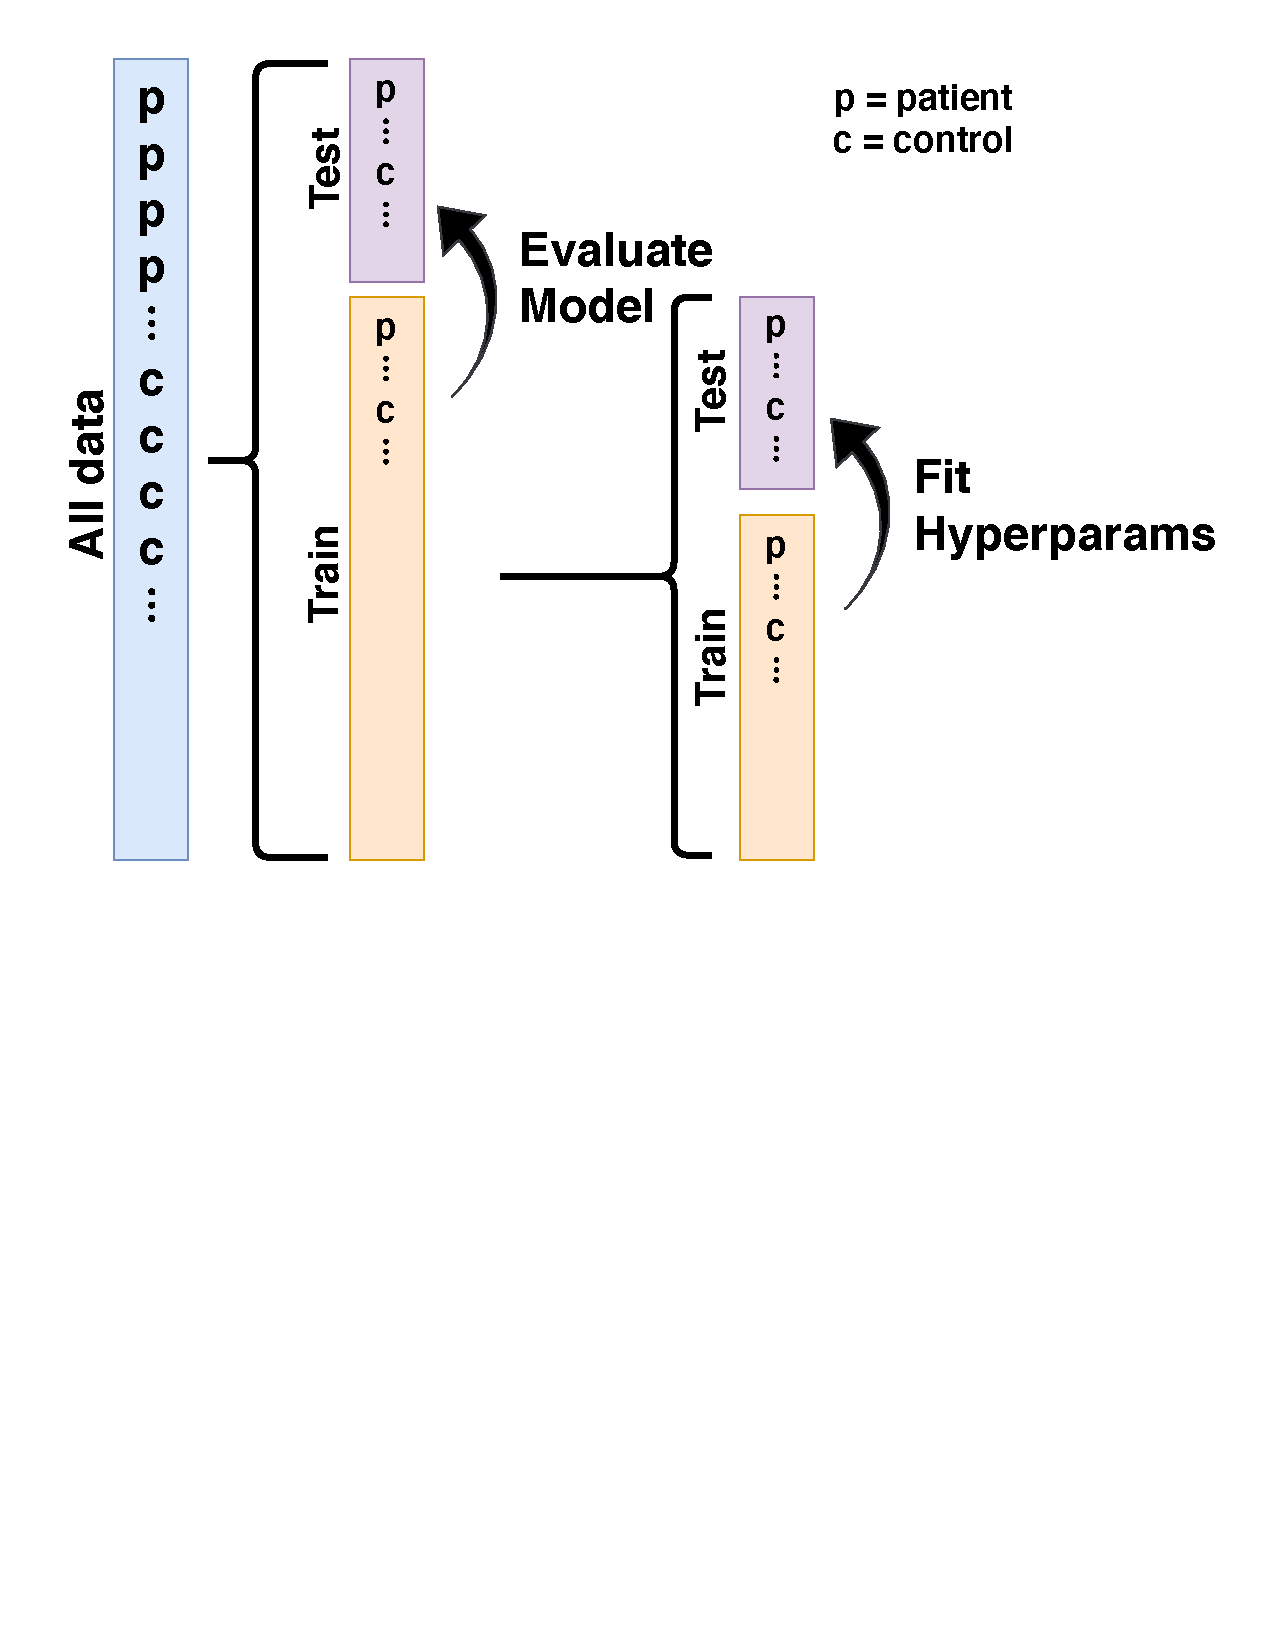
\includegraphics[width=0.75\textwidth]{nested-cross-validation.pdf}
    \caption{{\bf Nested cross-validation}
        \label{fig:nested-cross-val}
        We evaluate model quality using a nested $k$-fold cross validation
        scheme. At level-0, the input data is decomposed into $k_0$ shuffled
        groups and optimal hyperparameters are found for the level-0 training
        set. To avoid overfitting, the optimal hyperparameters are themselves
        evaluated using a cross-validation scheme taking place at level-1 of
        the decomposition, where each level-0 training set is further
        decomposed into $k_1 = 3$ shuffled groups. In the classification
        case, the training and test splits are stratified by diagnosis. For
        the ALS and WH data, $k_0 = 10$, while for the HBN and Cam-CAN data,
        $k_0 = 5$.
    }
\end{figure}

To objectively evaluate model performance and guard against over-fitting,
we used a nested cross-validation scheme, which is depicted for the binary
classification case in \cref{fig:nested-cross-val}. The subjects (i.e. rows
of the feature matrix $\mathbf{X}$ in \cref{fig:methods:group-structure}
and \cref{eq:lm}) are first shuffled and then decomposed into $k_0$ batches,
hereafter referred to as folds. For the ALS and WH datasets, we used $k_0 =
10$ and for the HBN and Cam-CAN datasets, $k_0 = 5$. For each unique fold, we
hold that fold out as the test\textsubscript{0} set and let the remaining
data comprise the train\textsubscript{0} set, with the subscript indicating
the depth of the nested decomposition. We further decompose each
train\textsubscript{0} set into three folds, and again for each unique fold,
we hold out that fold as the test\textsubscript{1} set and let the remaining
data comprise the train\textsubscript{1} set. At level-1 of the
decomposition, we fit an SGL model using fixed regularization meta-parameters
$\alpha$ and $\lambda$, training the model using train\textsubscript{1} and
evaluating the fit on test\textsubscript{1}. We find the optimal values for
$\alpha$ and $\lambda$ using sequential model-based optimization, implemented
using the scikit-optimize \lstinline|BayesSearchCV| class \cite{scikit_optimize}.
For continuous numerical $y$, \lstinline|BayesSearchCV| searches for
meta-parameter values that maximize the $R^2$ averaged over test sets. For
binary categorical $y$ \lstinline|BayesSearchCV| seeks to maximize the
classification accuracy. Using hyperoptimization, we find optimal
regularization parameters and $\hat{\beta}$ for each train\textsubscript{0}
set and then use those to predict values for data in test\textsubscript{0}.
Thus each subject in the dataset has a predicted phenotype derived from a
model that never saw its particular subject's data. In the classification
case, the shuffling into folds is stratified such that each fold has a
population that preserves the percentage of each class found in the larger
input data.

For each dataset, we also perform a randomization test by training similar
models on copies of the data for which the rows of the target variable $y$
have been shuffled while the feature matrix $\mathbf{X}$ remains the same.
This effectively destroys any relationship between the diffusion data and the
outcome. Indeed, all of our models perform no better than random guessing.
One should expect this since any better performance might indicate data
leakage between train and test sets \cite{kaufman2012leakage} or other common
machine learning pitfalls.

\subsection*{Software implementation}

The full software implementation of the SGL approach presented here is available
in a Python software package called \texttt{AFQ-Insight}, which is developed
publicly in \url{https://github.com/richford/afq-insight}.
The version of the code used to produce the results herein is also available in
\url{https://doi.org/10.5281/zenodo.4316000}.
AFQ-Insight reads the target and feature data that has been processed by AFQ
from comma separated value (CSV) files conforming to the AFQ-Browser data
format \cite{yeatman2018browser} and represents them internally as
\lstinline|DataFrame| objects from the pandas Python library
\cite{mckinney2010data}. The software provides different options for imputing
missing data in the feature matrix. Missing interior nodes are imputed using
linear interpolation. For missing exterior nodes, the user may choose between
linear extrapolation and constant forward- or back-fill. Imputation uses only
values from adjacent nodes in the same white matter bundle in the same
subject so there is no danger of data leakage from other subjects. It uses
the scikit-learn \cite{scikit-learn} library to decompose input data into
separate test and train datasets, to scale each feature to have zero mean and
unit variance, and to evaluate each fit in the hyperparameter search using
appropriate classification and regression metrics such as accuracy, area
under the receiver operating curve (AUC ROC), and coefficient of
determination ($R^2$). Internally, \texttt{AFQ-Insight} uses the
\texttt{groupyr} software library \cite{groupyr} mentioned above to solve the
SGL.

\section*{Supporting information}

% Include only the SI item label in the paragraph heading. Use the \nameref{label} command to cite SI items in the text.
\paragraph*{S1 Appendix.}
\label{S1_Appendix}
{\bf Bundle and regression coefficient profiles.}
In this supporting section, we present bundle profiles and $\hat{\beta}$ coefficients
for each anatomical bundle and in each dataset.

\section*{Acknowledgments}

This work was supported by BRAIN Iniative grant 1RF1MH121868-01 from the
National Institutes for Mental Health, by a grant from the Gordon \& Betty
Moore Foundation and the Alfred P. Sloan Foundation to the University of
Washington eScience Institute Data Science Environment, and by the Google
Cloud Platform Academic Research Credits Program. We would like to thank
Scott Murray for a useful discussion of the SGL method and Mareike Grotheer
\added{and John Kruper}
for helpful comments on the manuscript.

\nolinenumbers

\bibliography{paper}
% Compile your BiBTeX database using our plos2015.bst
% style file and paste the contents of your .bbl file
% here. See http://journals.plos.org/plosone/s/latex for
% step-by-step instructions.
\end{document}
